\documentclass[11pt]{article}

% Change "review" to "final" to generate the final (sometimes called camera-ready) version.
% Change to "preprint" to generate a non-anonymous version with page numbers.
\usepackage[final]{acl}

% Standard package includes
\usepackage{times}
\usepackage{latexsym}
\usepackage{graphicx} 
\usepackage{float}
\usepackage{stfloats}
\usepackage{placeins}
\usepackage{subcaption}
\usepackage{booktabs}

% For proper rendering and hyphenation of words containing Latin characters (including in bib files)
\usepackage[T1]{fontenc}
% For Vietnamese characters
% \usepackage[T5]{fontenc}
% See https://www.latex-project.org/help/documentation/encguide.pdf for other character sets

% This assumes your files are encoded as UTF8
\usepackage[utf8]{inputenc}

% This is not strictly necessary, and may be commented out,
% but it will improve the layout of the manuscript,
% and will typically save some space.
\usepackage{microtype}

% This is also not strictly necessary, and may be commented out.
% However, it will improve the aesthetics of text in
% the typewriter font.
\usepackage{inconsolata}

%Including images in your LaTeX document requires adding
%additional package(s)
\usepackage{graphicx}
\usepackage{amsmath}
\usepackage{float}
\usepackage{enumitem}
\usepackage{tabularx}

% If the title and author information does not fit in the area allocated, uncomment the following
%
%\setlength\titlebox{<dim>}
%
% and set <dim> to something 5cm or larger.

\title{Multiple Models for the NLI task}

% Author information can be set in various styles:
% For several authors from the same institution:
% \author{Author 1 \and ... \and Author n \\
%         Address line \\ ... \\ Address line}
% if the names do not fit well on one line use
%         Author 1 \\ {\bf Author 2} \\ ... \\ {\bf Author n} \\
% For authors from different institutions:
% \author{Author 1 \\ Address line \\  ... \\ Address line
%         \And  ... \And
%         Author n \\ Address line \\ ... \\ Address line}
% To start a separate ``row'' of authors use \AND, as in
% \author{Author 1 \\ Address line \\  ... \\ Address line
%         \AND
%         Author 2 \\ Address line \\ ... \\ Address line \And
%         Author 3 \\ Address line \\ ... \\ Address line}
\author{
\begin{tabular}{ccc}
\textbf{Zihan Wu} & \textbf{Jianyun Yang} & \textbf{Haoran Yu} \\
University of Western Australia & University of Western Australia & University of Western Australia \\
Perth, Australia & Perth, Australia & Perth, Australia \\
\texttt{24372276@student.uwa.edu.au} & \texttt{24181422@student.uwa.edu.au} & \texttt{24180266@student.uwa.edu.au}
\end{tabular}
}

%\author{
%  \textbf{First Author\textsuperscript{1}},
%  \textbf{Second Author\textsuperscript{1,2}},
%  \textbf{Third T. Author\textsuperscript{1}},
%  \textbf{Fourth Author\textsuperscript{1}},
%\\
%  \textbf{Fifth Author\textsuperscript{1,2}},
%  \textbf{Sixth Author\textsuperscript{1}},
%  \textbf{Seventh Author\textsuperscript{1}},
%  \textbf{Eighth Author \textsuperscript{1,2,3,4}},
%\\
%  \textbf{Ninth Author\textsuperscript{1}},
%  \textbf{Tenth Author\textsuperscript{1}},
%  \textbf{Eleventh E. Author\textsuperscript{1,2,3,4,5}},
%  \textbf{Twelfth Author\textsuperscript{1}},
%\\
%  \textbf{Thirteenth Author\textsuperscript{3}},
%  \textbf{Fourteenth F. Author\textsuperscript{2,4}},
%  \textbf{Fifteenth Author\textsuperscript{1}},
%  \textbf{Sixteenth Author\textsuperscript{1}},
%\\
%  \textbf{Seventeenth S. Author\textsuperscript{4,5}},
%  \textbf{Eighteenth Author\textsuperscript{3,4}},
%  \textbf{Nineteenth N. Author\textsuperscript{2,5}},
%  \textbf{Twentieth Author\textsuperscript{1}}
%\\
%\\
%  \textsuperscript{1}Affiliation 1,
%  \textsuperscript{2}Affiliation 2,
%  \textsuperscript{3}Affiliation 3,
%  \textsuperscript{4}Affiliation 4,
%  \textsuperscript{5}Affiliation 5
%\\
%  \small{
%    \textbf{Correspondence:} \href{mailto:email@domain}{email@domain}
%  }
%}

\begin{document}
\maketitle
\begin{abstract}
Natural Language Inference (NLI) is a fundamental task in natural language understanding that aims to determine the logical relationship between a pair of sentences — typically identifying whether a hypothesis is entailed, contradicted, or neutral with respect to a premise. This study investigates and compares three neural architectures for the NLI task: a Bidirectional Long Short-Term Memory (BiLSTM) model, an Encoder–Decoder model with an LSTM encoder and GRU decoder, and a Transformer-based model. The BiLSTM serves as a baseline for sequential modeling, while the Encoder–Decoder model explores cross-sequence representation learning, and the Transformer model leverages global attention mechanisms for contextual understanding. Experiments were conducted on a benchmark NLI dataset to evaluate classification performance and generalization ability. The results show that the Transformer-based model achieves the highest overall accuracy , confirming its superior ability to model long-range dependencies and semantic nuances. The LSTM–GRU encoder–decoder model demonstrates moderate improvement over BiLSTM, indicating that hybrid recurrent structures with attention can enhance representation learning. These findings highlight the progressive effectiveness of attention mechanisms and non-recurrent architectures for natural language reasoning tasks.
\end{abstract}

\section{Introduction}
Natural Language Inference (NLI), also known as Recognizing Textual Entailment (RTE), is a core problem in natural language understanding. The task involves determining whether a given hypothesis can be logically inferred from a premise sentence, or whether the relationship between them is one of entailment, contradiction, or neutrality. NLI plays an essential role in applications such as question answering, dialogue systems, information retrieval, and text summarization, where understanding sentence-level meaning and reasoning is crucial.

Early NLI systems relied heavily on hand-crafted linguistic features, syntactic rules, or lexical resources. However, such approaches often struggled to capture the subtleties of context and semantics in natural language. With the rise of deep learning, neural network models have become the dominant approach, capable of automatically learning distributed representations of words and sentences. Despite this progress, the choice of architecture significantly influences model performance, as different networks capture context and dependencies in distinct ways.And there are several models that are commonly used in the NLI tasks, which are  RNN-based model and Transformer-based models.

This paper presents a comparative analysis of three representative neural architectures for the NLI task: a Bidirectional LSTM (BiLSTM), an Encoder–Decoder model combining an LSTM encoder and GRU decoder, and a Transformer-based model. The BiLSTM provides a sequential baseline that processes input in both temporal directions, capturing local context efficiently. The LSTM–GRU Encoder–Decoder model introduces a hierarchical structure that can learn complex inter-sentence representations through sequence-to-sequence processing. Finally, the Transformer model applies multi-head self-attention to capture global dependencies without recurrence, offering the potential for improved reasoning over longer contexts.

Compared to existing methods of multiple papers, we have applied some updates into our models
The innovation of the BiLSTM model lies in the integration of multiple attention mechanisms to explore how different attention strategies influence the model’s ability to align and interpret semantic relations between the premise and hypothesis. This design enables a deeper understanding of which contextual cues are most critical for entailment recognition.
The LSTM–GRU Encoder–Decoder model introduces the GRU as the decoder to reduce the computational overhead of traditional LSTM-based decoders while maintaining competitive representational capacity. This hybrid architecture allows efficient gradient propagation and faster convergence, making it suitable for NLI tasks with large sentence pairs.
Lastly, the Transformer-based model departs from conventional encoder-focused designs by employing the Transformer architecture in the decoder stage. This modification allows the model to enhance interpretive reasoning in the final inference stage, leveraging attention-based decoding to better integrate semantic relationships between encoded premise–hypothesis representations.


\section{Methods}
\subsection{Model A——BILSTM encoding only}
In this model, we use BILSTM encoding only to train the dataset. BiLSTM is Bidirectional Long Short-Term Memory model which considers the forward stream of data and backward stream of data at the same time.

\paragraph{Architecture}The input part for this model is the embedded vector.Suppose the embedded vector of premise and hypothesis are 
\begin{align}
\mathbf{E}_P &= [\mathbf{e}_{p_1}, \mathbf{e}_{p_2}, \dots, \mathbf{e}_{p_m}] \in \mathbb{R}^{m \times 100} \\
\mathbf{E}_H &= [\mathbf{e}_{h_1}, \mathbf{e}_{h_2}, \dots, \mathbf{e}_{h_n}] \in \mathbb{R}^{n \times 100}
\end{align}

Then, we use LSTM to encode vector with considering the hidden state from forward and backward
\begin{align} 
\overrightarrow{\mathbf{h_t}} &= \text{LSTM}(e_{p_t}, \overrightarrow{h_{t-1}})\\ 
\overleftarrow{\mathbf{h_t}} &= \text{LSTM}(e_{p_t}, \overleftarrow{h_{t+1}}) 
\end{align}
The hidden state at position t is the concatenation of both directions:
\begin{align} 
\mathbf h_t = [\overrightarrow{h_t}; \overleftarrow{h_t}] \in \mathbb{R}^{256}
\end{align}
The complete BiLSTM outputs are:
\begin{align} 
\mathbf O_P = [h_1, h_2, \dots, h_m] \in \mathbb{R}^{m \times 256}\\
\mathbf O_H = [h_1, h_2, \dots, h_n] \in \mathbb{R}^{n \times 256}
\end{align}

Then,we applied the attention mechanism.The attention mechanism assigns weights to each hidden state to highlight the most relevant parts of the sequence. For each time step t, the attention score st is computed using a linear transformation:
\begin{align} 
\mathbf s_t = W_a h_t + b_a
\end{align}
where $W_a \in \mathbb{R}^{256 \times 1}$ and $b_a \in \mathbb{R}$.

Attention weights $\alpha_t$ are obtained via the softmax normalization:
\begin{align} 
\mathbf \alpha_t = \frac{\exp(s_t)}{\sum_{t'=1}^{m} \exp(s_{t'})}
\end{align}
The attended representation of the premise and the attended representation of the hypothesis should be 
\begin{align} 
\mathbf a_P = \sum_{t=1}^{m} \alpha_t h_t \in \mathbb{R}^{256}\\
\mathbf a_H = \sum_{t=1}^{n} \beta_t h_t \in \mathbb{R}^{256}
\end{align}
The attended vectors of the premise and hypothesis are concatenated and passed through
a fully connected layer to predict the relationship label and The output logit o is converted into a probability using the sigmoid function
\begin{align} 
\mathbf c &= [a_P; a_H] \in \mathbb{R}^{512} \\
\mathbf o &= W_f c + b_f \\
\mathbf p &= \sigma(o) = \frac{1}{1 + e^{-o}}
\end{align}
\subsection{Model B: Encoder--Decoder with Cross-Attention}
Model B is designed to capture complex relationships between premise and hypothesis using an encoder--decoder framework with cross-attention. The encoder is a single-layer bidirectional LSTM (BiLSTM) that encodes the premise. The decoder is a single-layer GRU that generates the hypothesis representation, attending to the encoded premise at each step via dot-product cross-attention.

\paragraph{Architecture}
Let $P = (p_1, \ldots, p_{n_p})$ be the premise token sequence and $H = (h_1, \ldots, h_{n_h})$ the hypothesis. The premise is embedded and encoded as $\mathbf{E}_P = \mathrm{BiLSTM}(\mathrm{Embed}(P))$. The decoder GRU processes the hypothesis tokens, and at each step $t$, computes attention weights $\alpha_t = \mathrm{softmax}(\mathbf{E}_P \cdot \mathbf{q}_t)$, where $\mathbf{q}_t$ is the decoder hidden state. The context vector $\mathbf{c}_t = \sum_i \alpha_{t,i} \mathbf{E}_{P,i}$ is concatenated with the decoder input.

\paragraph{Pooling Strategies}
To obtain a fixed-size sentence representation, we ablate four pooling methods over the encoder outputs: mean pooling, max pooling, last hidden state, and a learned query vector (attention pooling). The pooled vector is used for final classification.

\paragraph{Equations}
\begin{align}
\mathbf{E}_P &= \mathrm{BiLSTM}(\mathrm{Embed}(P)) \\
\mathbf{q}_t &= \mathrm{GRU}(h_{t-1}, y_{t-1}) \\
\alpha_t &= \mathrm{softmax}(\mathbf{E}_P \cdot \mathbf{q}_t) \\
\mathbf{c}_t &= \sum_i \alpha_{t,i} \mathbf{E}_{P,i}
\end{align}

\subsection{Model C: Decode-only Transformer with Disentangled Self-Attention}
\label{sec:methods-danli}

\paragraph{Architecture Overview}
We concatenate the premise and hypothesis and pass them through a decoder-only Transformer stack with a disentangled self-attention module that separates content (token embeddings) from position (sinusoidal features). Instead of adding positions to tokens, we keep them separate and learn distinct projections for content vs.\ position. After the stack, we split the sequence back into premise/hypothesis spans, apply masked mean pooling over each span, combine the two vectors with standard NLI matching features, and classify with a small MLP.

\paragraph{Disentangled Multi-Head Self-Attention}
Gaining insight from this paper\cite{he2020deberta}, attention logits are the sum of three terms  instead of one content$\leftrightarrow$content score:
\begin{itemize}
 \textbf{c2c}: content$\to$content
 \textbf{c2p}: content$\to$position 
 \textbf{p2c}: position$\to$content 
\end{itemize}
Values still come from content. Position is never added to token embeddings, it only influences how attention is aimed.

\begin{align}
\mathbf{q}^{(c)}_t&=W^{(c)}_Q \mathbf{x}_t,&
\mathbf{k}^{(c)}_t&=W^{(c)}_K \mathbf{x}_t,&
\mathbf{v}^{(c)}_t&=W^{(c)}_V \mathbf{x}_t,\\
\mathbf{q}^{(p)}_t&=W^{(p)}_Q \mathbf{r}_t,&
\mathbf{k}^{(p)}_t&=W^{(p)}_K \mathbf{r}_t. &&
\end{align}
The attention score from position $i$ (query) to $j$ (key) is
\begin{equation}
s_{ij}
= \frac{
\langle \mathbf{q}^{(c)}_i, \mathbf{k}^{(c)}_j\rangle
+ \langle \mathbf{q}^{(c)}_i, \mathbf{k}^{(p)}_j\rangle
+ \langle \mathbf{q}^{(p)}_i, \mathbf{k}^{(c)}_j\rangle
}{\sqrt{d_h}}
\end{equation}
The padding mask prevents attention to placeholder PAD tokens. We then apply the softmax function to the masked scores to convert them into a valid probability distribution, which represents as the attention weights (A).
We then apply a linear projection, dropout, and the usual residual--norm and FFN sublayers per Transformer block.


\emph{Positional Features}
For time step $t$ (0-indexed), the sinusoidal positional vector $\mathbf{r}_t \in \mathbb{R}^{d}$ uses the standard $\sin/\cos$ basis. We apply dropout to $\{\mathbf{r}_t\}$ and do not add it to token embeddings.
\emph{Span Pooling and NLI Head}
After the stack, split the sequence back into premise and hypothesis spans. Do masked mean-pooling on each span to get two vectors.
Build [p, h, |p–h|, $[p\odot h]$] and pass through a small MLP to get a single logit, then probability.

\paragraph{Justification for the Design}
\emph{Disentangling content and position:} it helps separate token semantics from positional information, which allows the model to capture lexical relationships and the relative placement of evidence.
\emph{Decoder-only:} it lets the hypothesis attend to earlier premise tokens within one stream, which simplify implementation and improving efficiency.

\section{Experiment Setup}
\subsection{Dataset Description}
\noindent The dataset is divided into three splits:
\begin{itemize}[leftmargin=1em, itemsep=0pt, topsep=0pt]
    \item \textbf{Training split} (\texttt{train.json}): Contains 23,088 examples (indices 0--23,087), with approximately 45\% ``entails'' and 55\% ``neutral'' labels (rough estimate based on the excerpt).
    \item \textbf{Validation split} (\texttt{validation.json}): Contains 1,304 examples (indices 0--1,303), with roughly 48\% ``entails'' and 52\% ``neutral'' labels.
    \item \textbf{Overall distribution:} About 46\% ``entails'' and 54\% ``neutral'' across the dataset.
\end{itemize}

\begin{table}[H]
  \centering
  \begin{tabular}{lcc}
    \hline
    \textbf{Split} & \textbf{Examples} & \textbf{Labels (\% E/N)} \\
    \hline
    Train & 23,088 & 45 / 55 \\
    Validation & 1,304 & 48 / 52 \\
    Test & 2,126 & 46 / 54 \\
    \hline
  \end{tabular}
  \hfill
  \begin{tabular}{lcc}
    \hline
    \textbf{Split} & \textbf{Min Tokens} & \textbf{Max Tokens} \\
    \hline
    Train & 4 & 30 \\
    Validation & 16 & 44 \\
    Test & 2 & 41 \\
    \hline
  \end{tabular}
  \caption{Dataset statistics and token counts for training, validation, and test splits.}
  \label{tab:dataset_stats}
\end{table}
\subsection{Implementation Details}
\paragraph{Model Configuration}For model A and B, we applied the same configuration parameters to them.We set the hidden size to 128 and embedding dimension to 100.
\begin{table}[h]
\centering
\small
\begin{tabular}{p{2.8cm}l}
\hline
Hyperparameter & Value \\
\hline
embedding dimension & 100\\
Hidden dimension & 128 \\
Dropout rate & 0.2 \\
Pooling types & mean, max, last, attention \\
Learning rate & $1\times10^{-3}$ \\
Batch size & 32 \\
Epochs & 3 \\
Patience & 2 \\
Max sequence length & 50 \\
\hline
\end{tabular}
\caption{Model A and B configuration and hyperparameters.}
\label{tab:modelb-config}
\end{table}

For model C-Transformer: $N{=}4$ decoder layers, $d_{\text{model}}{=}256$, $n_{\text{heads}}{=}8$, FFN hidden $=512$. Disentangled attention dropout $0.2$; sinusoidal feature dropout $0.2$. Classifier: MLP $4d \rightarrow d \rightarrow 1$ with ReLU and dropout $0.2$. Masks: causal over the concatenated sequence; key padding mask for pads. Pooling: masked mean per span.    Training-Loss: \texttt{BCEWithLogitsLoss}. Optimizer: Adam, LR $1{\times}10^{-4}$. batch size: 32. Train up to 10 epochs with early stopping; patience: 2 on validation accuracy. 

\section{Result}
\subsection {Main Performance Comparison}
In this part, we compare the accuracy score of these three models in the test data set. The outcome shows that for model A, B,and c, the accuracy score are 0.69285,0.7262,0.76783

\begin{table}[H]
  \centering
  \begin{tabular}{lcc}
    \hline
    \textbf{Model} & \textbf{Accuracy} \\
    \hline
    BILSTM & 0.69285  \\
    BILSTM-GRU & 0.7262 \\
    Transformer-based & 0.76783 \\
    \hline
  \end{tabular}
  \caption{Accuracy for different model.}
\end{table}
This result fits for what we expected, since The model C - transformer-based model achieves the best performance.And the reason why Transformer-based model achieves the highest accuracy is because its self-attention mechanism captures global contextual dependencies more effectively than sequential models like BiLSTM and BiLSTM-GRU, enabling richer feature representation and better generalization.
\subsection {Ablation study for attention}
In this part, we applied four different attention format for BILSTM model to test which one is the best, which are Self-attention, dot-attention, general-attention and additive-attention. For more math details, refer to \textbf{Appendix A}
\paragraph{Self-Attention.}
Each word in the sentence “attends” to itself.the model learns which tokens within the same sentence are more important when forming a sentence-level representation.

\paragraph{Dot-Product Attention.}
Measures interaction between two sequences (the premise and hypothesis) using a simple dot product. It tells the model how well each token in the premise aligns with each token in the hypothesis.
\paragraph{General Attention.}
A generalization of dot-product attention that includes a learnable linear transformation before computing similarity.
\paragraph{Additive (Bahdanau) Attention.}
Instead of using dot products, it learns a small feed-forward neural network to compute attention scores.Additive attention learns nonlinear relationships between tokens in the premise and hypothesis, rather than just relying on dot products.
\begin{table}[H]
  \centering
  \begin{tabular}{lcc}
    \hline
    \textbf{Attention Type} & \textbf{Accuracy}  \\
    \hline
    Self & 0.681  \\
    Dot & 0.697  \\
    General & 0.692  \\
    Additive & 0.705 \\
    \hline
  \end{tabular}
  \caption{different Attention type accuracy comparison}
  \label{tab:dataset_stats}
\end{table}

We also study how cross content--position interactions shape performance by ablating the \texttt{c2p} and \texttt{p2c} in the disentangled attention logits on model C (variants equation refers to Appendix B).
The result (table 5) shows that \texttt{full} model has the best performance on accuracy(0.767), followed by \texttt{c2p\_p2c} (0.762), \texttt{c2p\_only} (0.754), and \texttt{p2c\_only} (0.680). 
Overall, the \texttt{full} model achieves the highest test accuracy but tend to train longer.
Both \texttt{c2p\_only} and \texttt{c2p\_p2c} train faster, with a acceptable drop in accuracy.
The result also suggests that \texttt{c2p} is more useful than \texttt{p2c}: the \texttt{p2c\_only}
variant performs worst, while \texttt{c2p\_only} remains as a competitive model.
\FloatBarrier
\begin{table}[H]
\centering
\caption{Test accuracy with deltas vs.\ \texttt{full}}
\label{tab:attn-ablation-acc}
\begingroup
\footnotesize                 % or \scriptsize
\setlength{\tabcolsep}{4pt}   % default ~6pt
\renewcommand{\arraystretch}{0.95} % tighten row height
\begin{tabular}{lcc}
\toprule
Mode & Test Acc & $\Delta$Test vs.\ Full \\
\midrule
\texttt{full}      & \textbf{0.767} & +0.0000 \\
\texttt{c2p\_only} & 0.754          & $-0.0122$ \\
\texttt{p2c\_only} & 0.680          & $-0.0870$ \\
\texttt{c2p\_p2c}  & 0.762          & $-0.0042$ \\
\bottomrule
\end{tabular}
\endgroup
\end{table}
\FloatBarrier

\subsection {Additional Ablation study}
In this part, we did a Additional Ablation study for BILSTM model by changing the hidden size from 64 o 256, which is we used three values as a hidden size list [64,128,256]. In this part, we combined different attention mechanisms and different hidden size, then calculate the average accuracy of diffrent attention mechanisms. The outcome shows when hidden layer is 256, it will get the highest accuracy, which is 0.7135
\begin{table}[H]
  \centering
  \begin{tabular}{lcc}
    \hline
    \textbf{Hidden Size} & \textbf{Accuracy}  \\
    \hline
    64 & 0.681  \\
    128 & 0.694  \\
    256 & 0.7135  \\
    \hline
  \end{tabular}
  \hfill
  \caption{different hidden size accuracy comparison}
  \label{tab:dataset_stats}
\end{table}
That makes sense since when hidden layer becomes bigger, it will catch more possible features of the model and make it more accurate when other parameters keep same.
\section{Qualititive Study}
We select one test-set example for qualitative analysis on model C and extract attention weights for a true positive (TP) and a false positive (FP). The results(here just display two variants, other two refers to appendix C) show that all variants concentrate hypothesis$\!\to\!$premise (H$\!\to\!$P) attention on a small set of premise columns, and yield high--confidence correct decisions on entailment cases. In neutral cases with high surface overlap but different logic (e.g., negation or conditionals), attention clings to overlapping words and underweights logical composition, which leads to false--positive predictions. Models that include cross terms---especially \(\mathrm{C}\!\to\!\mathrm{P} + \mathrm{P}\!\to\!\mathrm{C}\)---tend to be more conservative on FPs and help reduce overconfidence.
\FloatBarrier


% ---------- P→C only: TP vs FP ----------
\begin{figure}[!htbp]
  \centering
  \begin{subfigure}{0.49\linewidth}
    \centering
    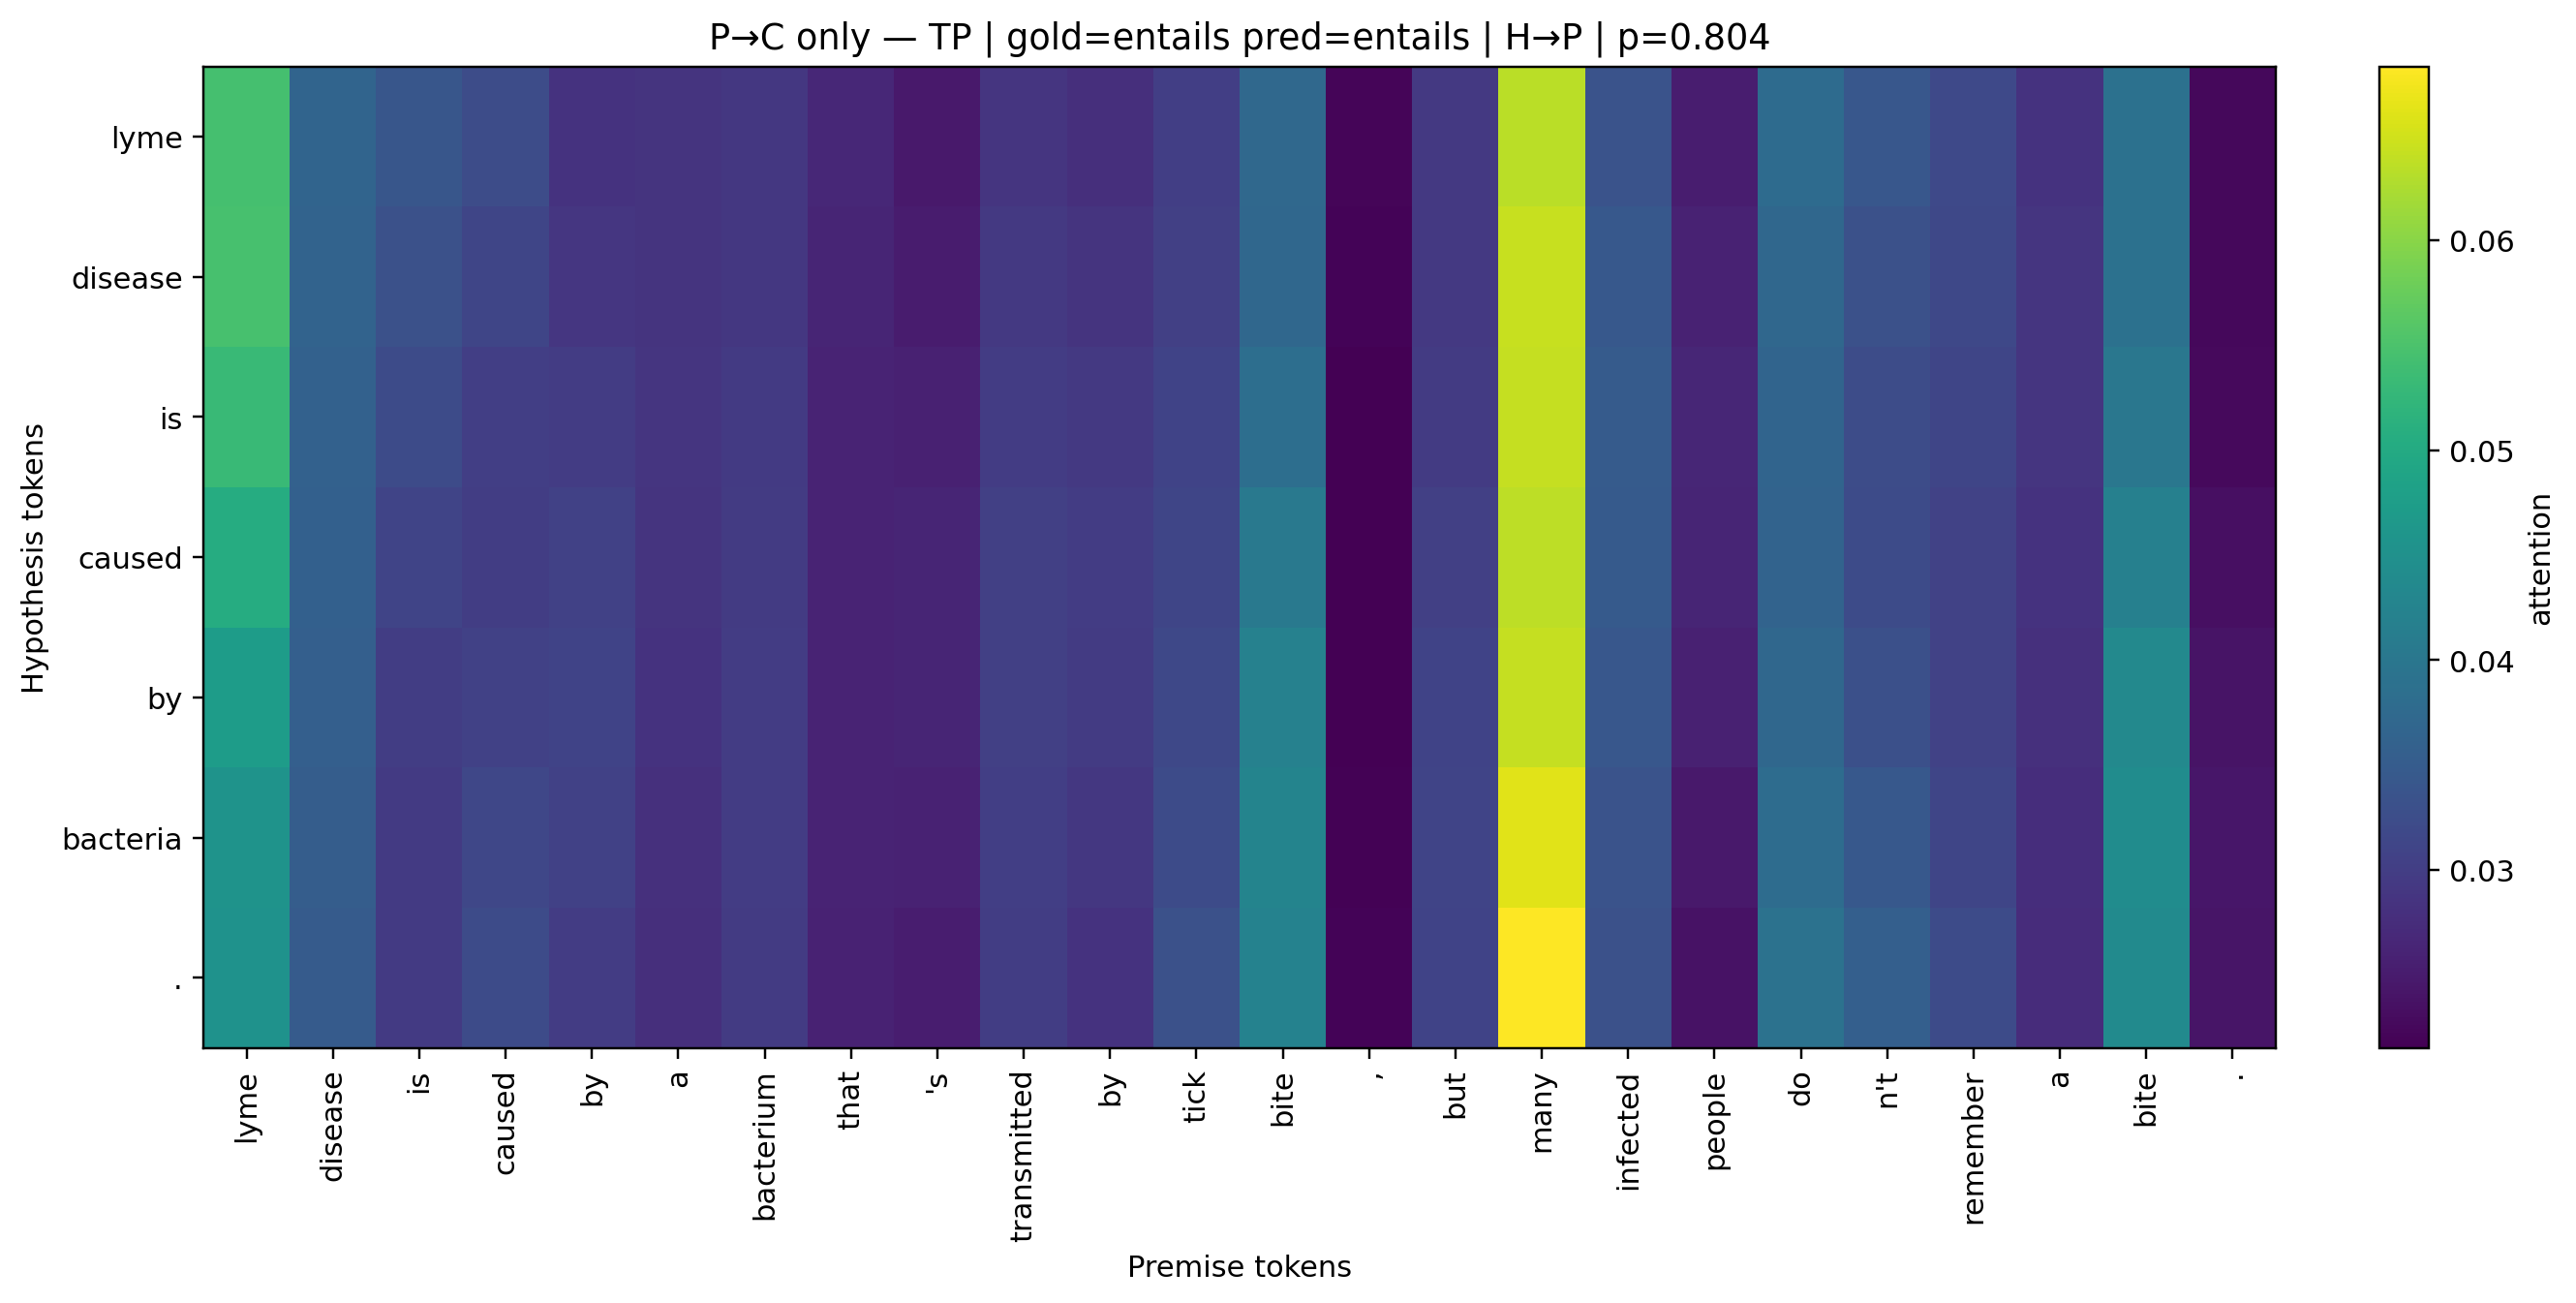
\includegraphics[width=\linewidth]{p2c_only_TP_y-entails_pred-entails_p-0.804_H2P.png}
    \caption{P$\to$C only — TP}
    \label{fig:p2c-tp}
  \end{subfigure}\hfill
  \begin{subfigure}{0.49\linewidth}
    \centering
    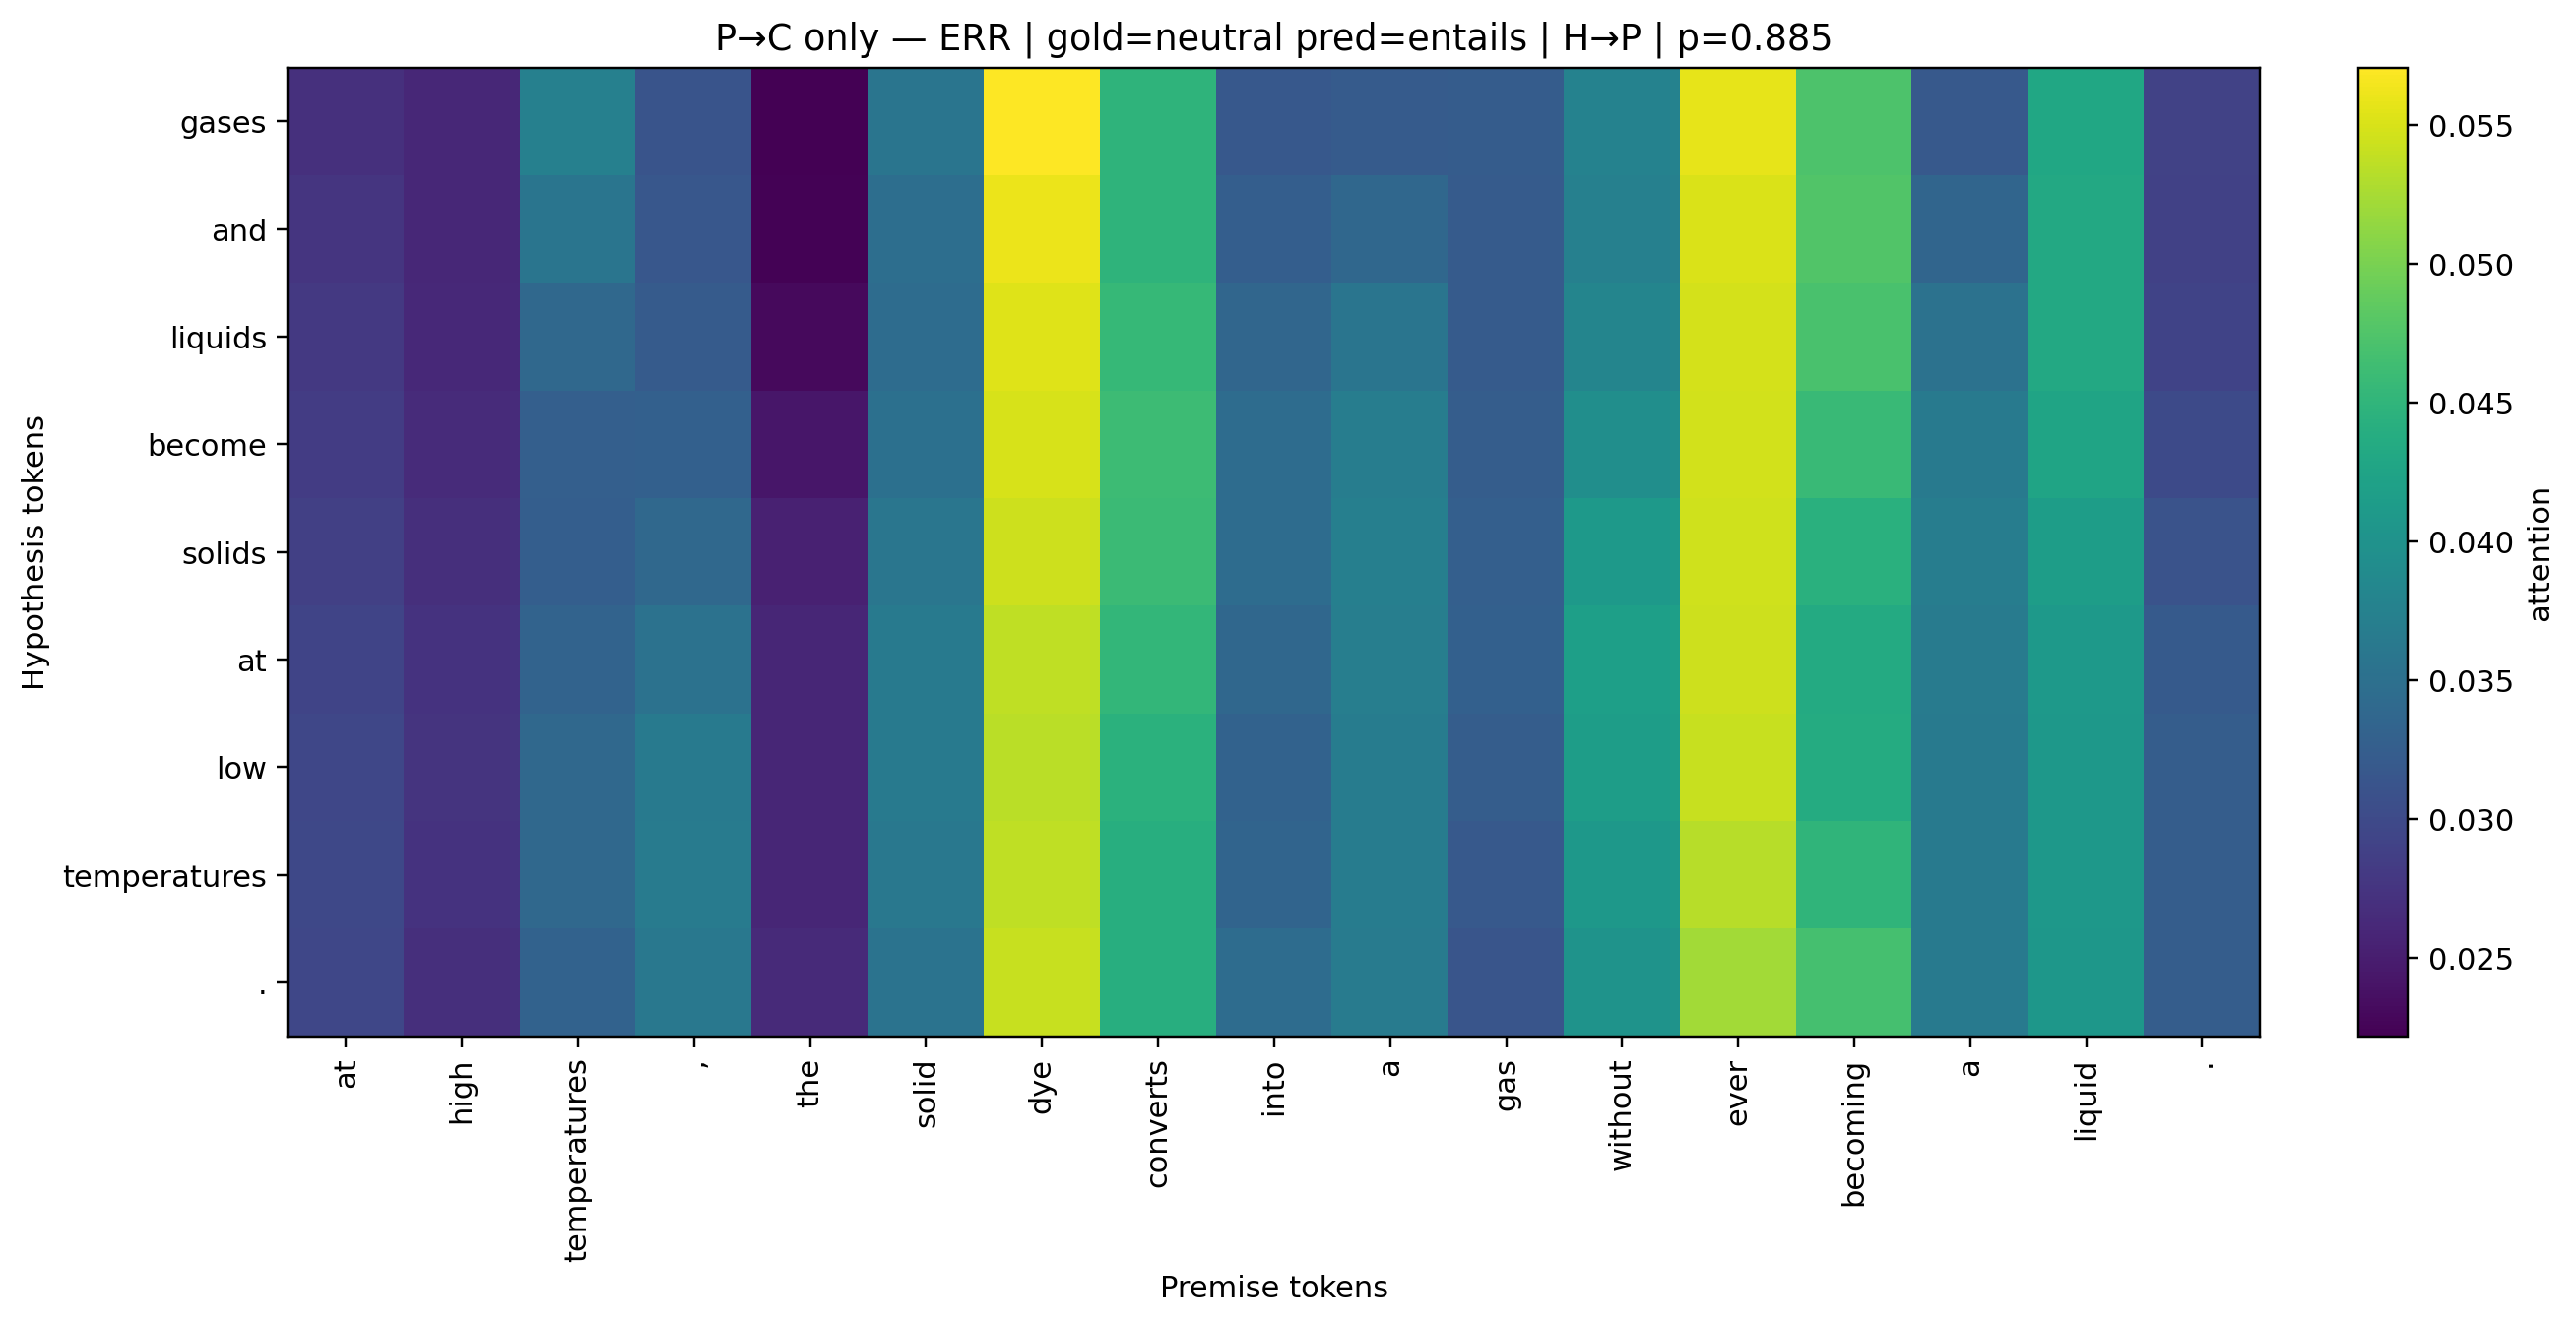
\includegraphics[width=\linewidth]{p2c_only_ERR_y-neutral_pred-entails_p-0.885_H2P.png}
    \caption{P$\to$C only — FP}
    \label{fig:p2c-fp}
  \end{subfigure}
  \caption{\textit{P$\to$C only} model: TP vs.~FP.}
  \label{fig:p2c-pair}
\end{figure}

% ---------- C→P + P→C: TP vs FP ----------
\begin{figure}[!htbp]
  \centering
  \begin{subfigure}{0.49\linewidth}
    \centering
    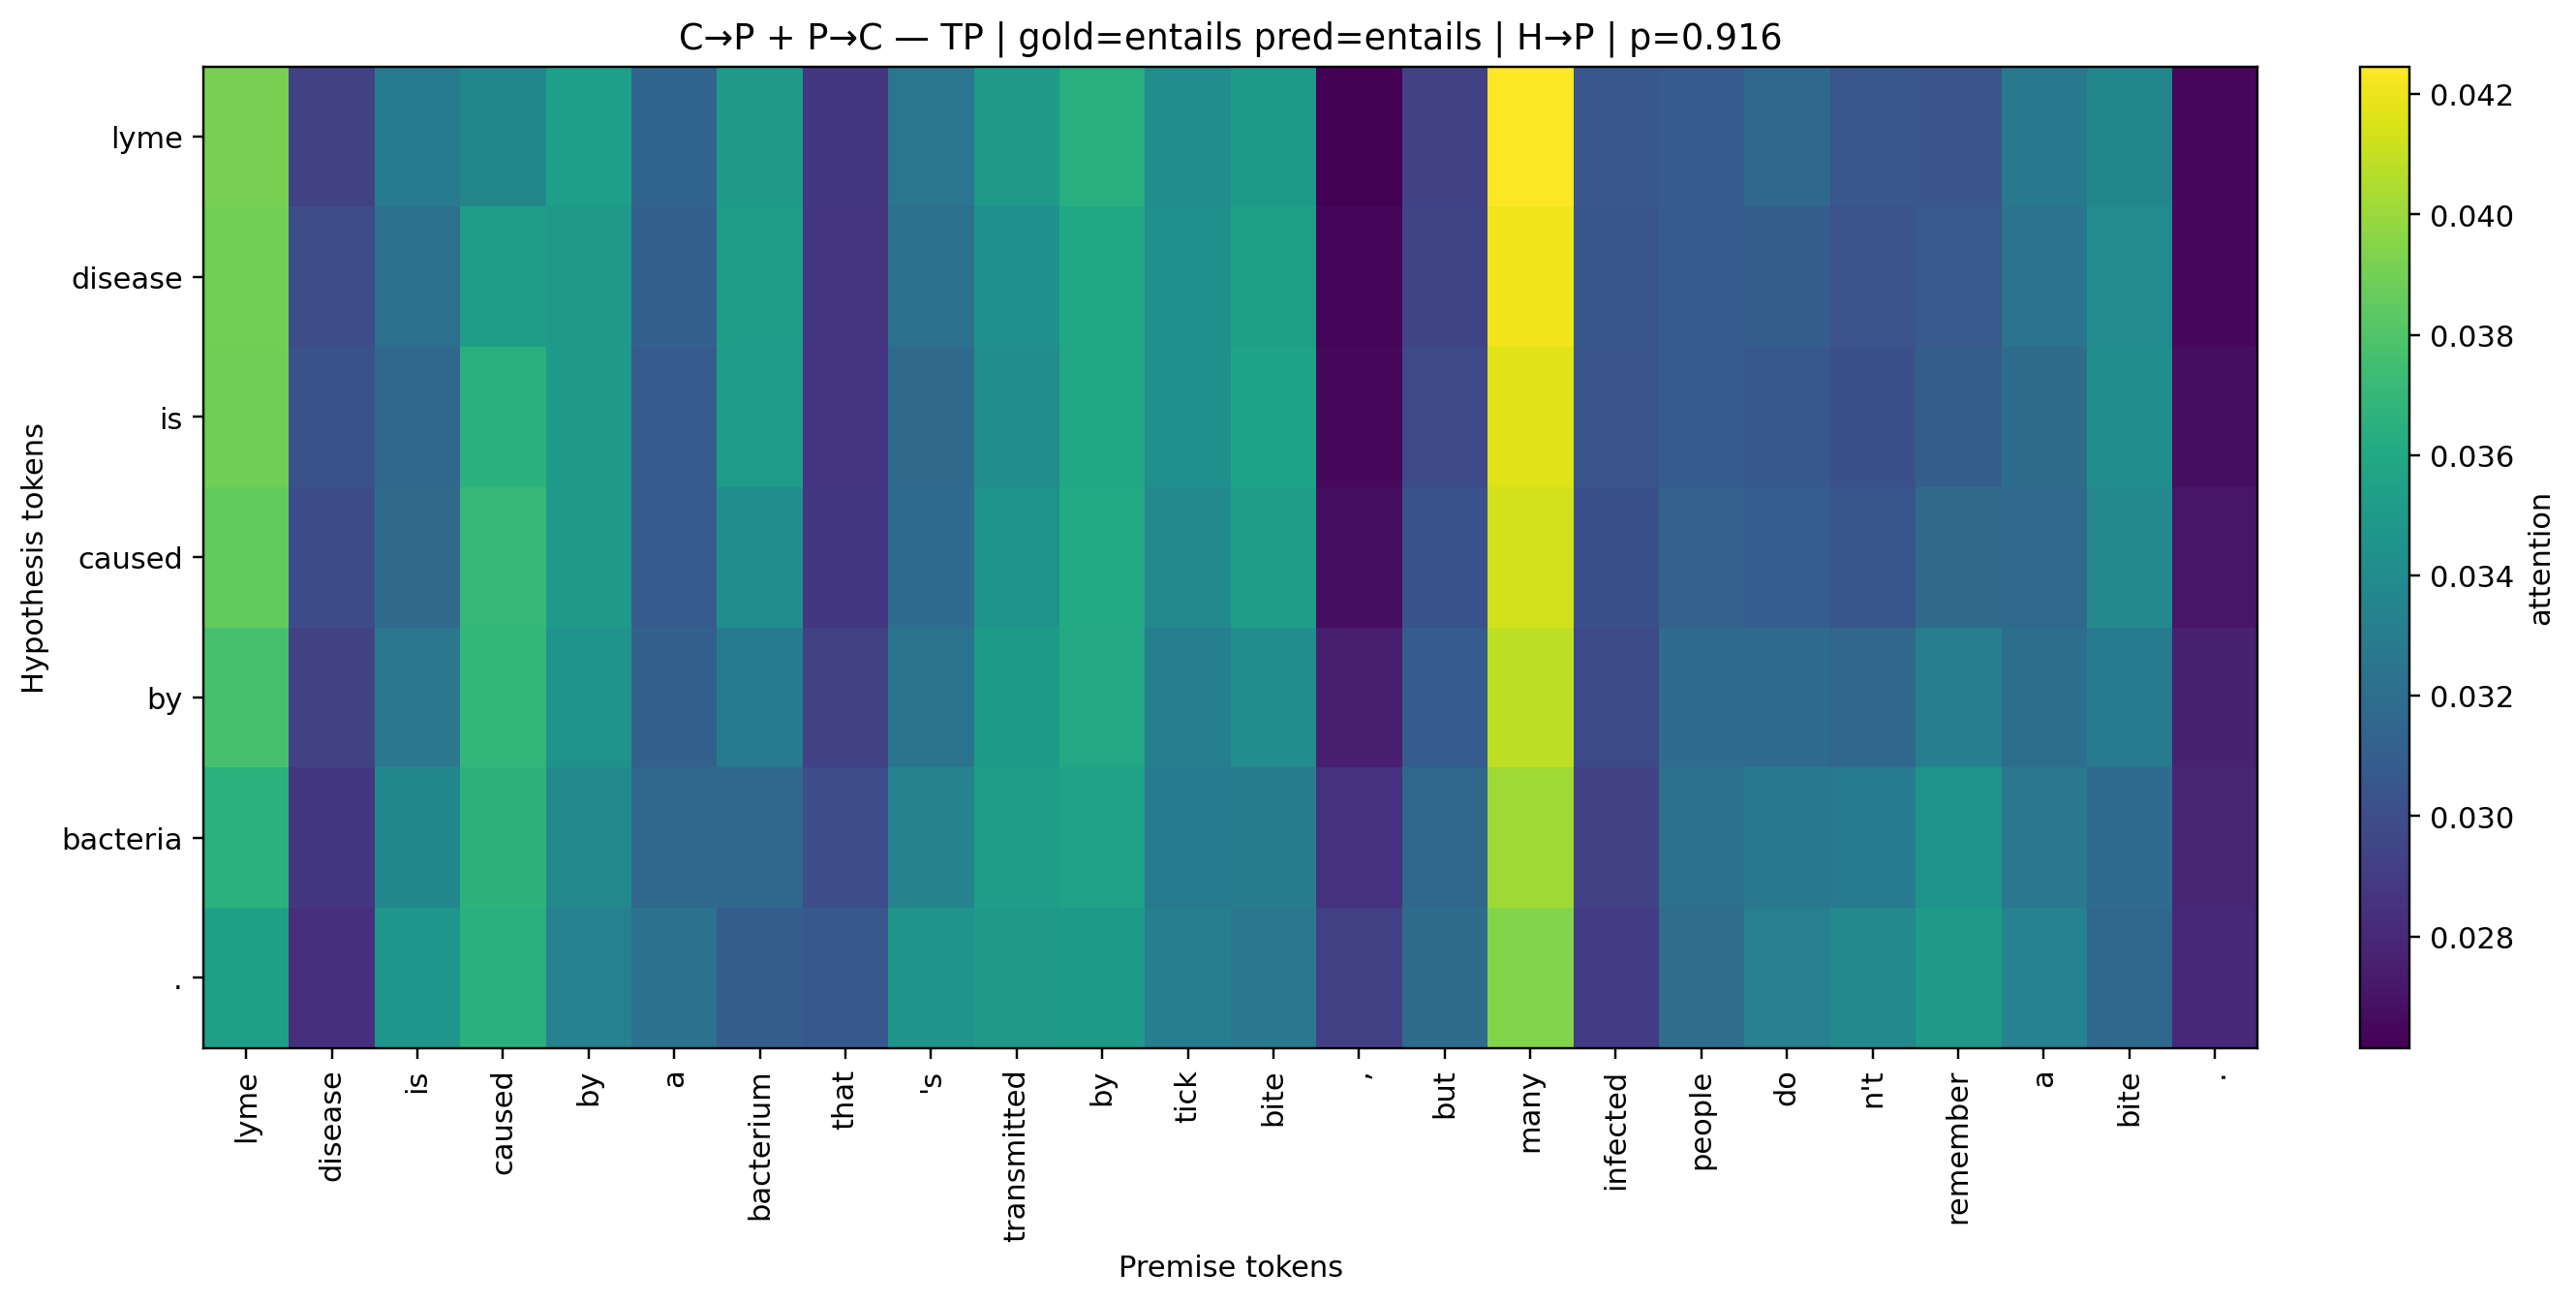
\includegraphics[width=\linewidth]{c2p_p2c_TP_y-entails_pred-entails_p-0.916_H2P.png}
    \caption{C$\to$P + P$\to$C — TP}
    \label{fig:c2pp2c-tp}
  \end{subfigure}\hfill
  \begin{subfigure}{0.49\linewidth}
    \centering
    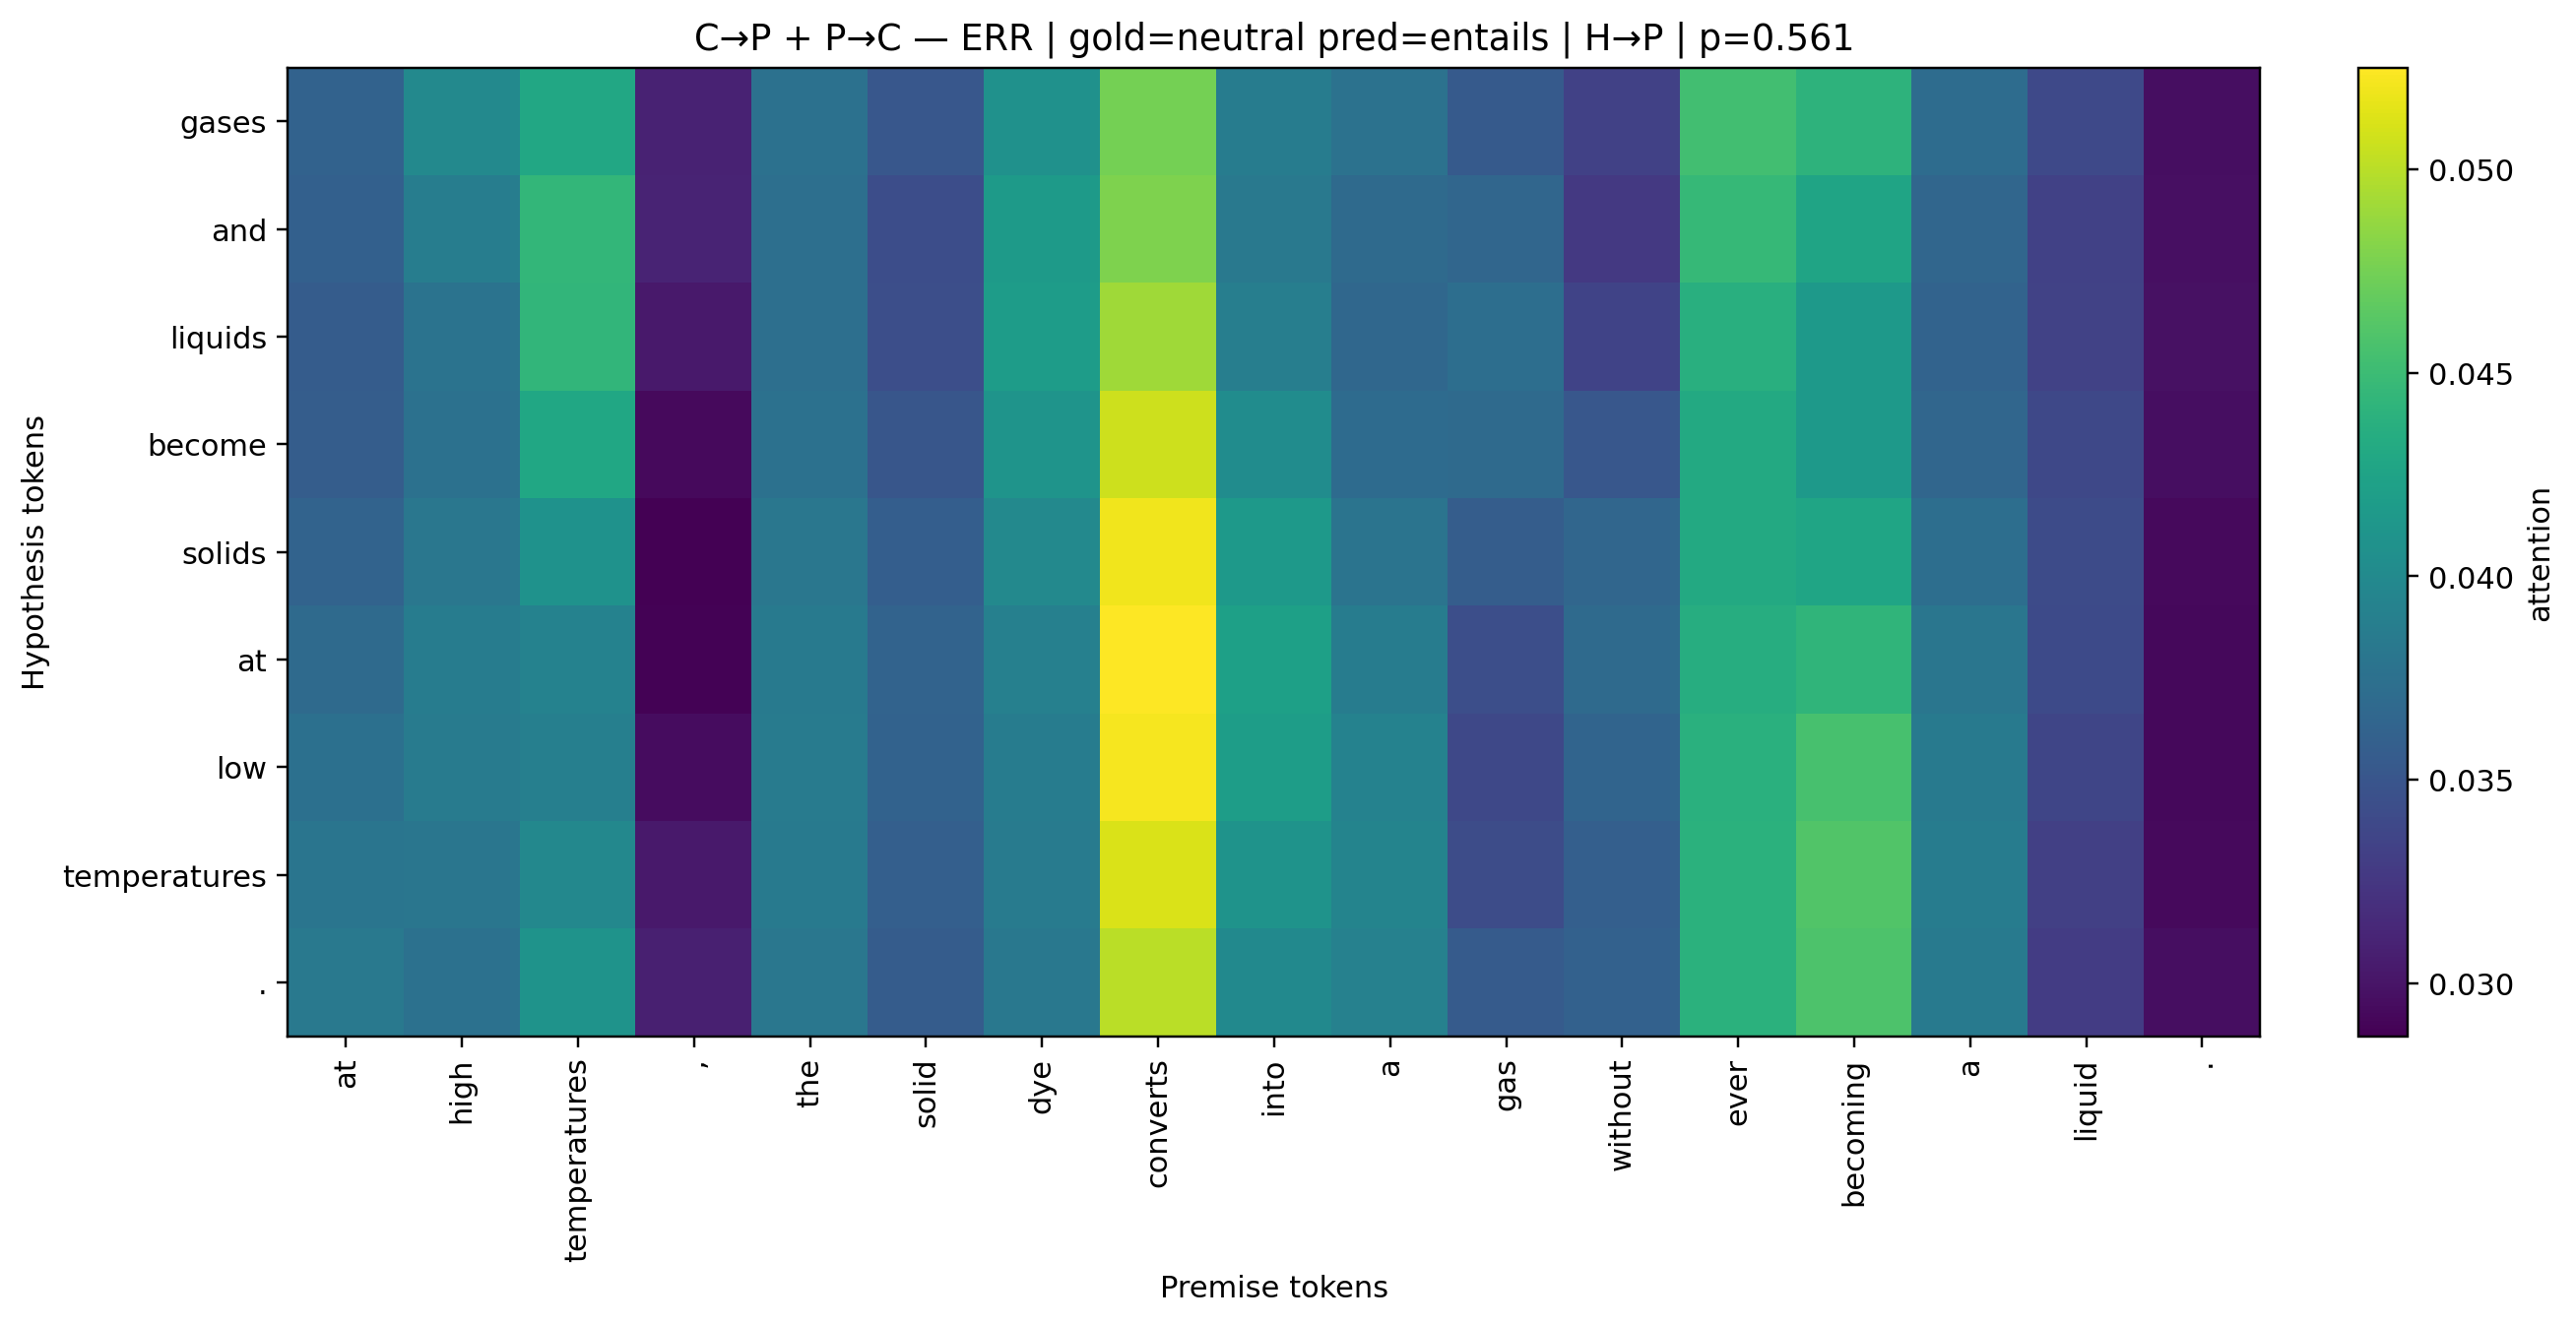
\includegraphics[width=\linewidth]{c2p_p2c_ERR_y-neutral_pred-entails_p-0.561_H2P.png}
    \caption{C$\to$P + P$\to$C — FP}
    \label{fig:c2pp2c-fp}
  \end{subfigure}
  \caption{C$\to$P + P$\to$C: TP vs.~FP.}
  \label{fig:c2pp2c-pair}
\end{figure}

\FloatBarrier

\section{Conclusion}
In this project, we have built three models with different architectures: BiLSTM, an LSTM-GRU encoder-decoder, and a decoder-only Transformer with disentangled self-attention. The Transformer-based model has the highest test accuracy (0.7678). The attention ablation studies indicate that additive attention performed best (0.705), and additional ablation studies show that increasing the BiLSTM hidden size to 256 improved average accuracy to 0.7135. Disentangled-attention ablations clarified the role of cross terms: \texttt{full} achieved the top accuracy while \texttt{p2c\_only} performed worst, suggesting \texttt{c2p} is more useful than \texttt{p2c}. The lighter variants trained faster with small drops in accuracy for efficiency. Our qualitative analysis indicates that our transformer models tend to be overconfident on entailment when there is high lexical overlap with different logic. But content-to-position and position-to-content cross terms help model be conservative. Overall, we found that choosing the right architecture and being able to model cross-terms interactions are more important than fine-tuning hyperparameters. Our main achievements were building three different architecture models and conducting various types of studies on their performance and behaviors, running targeted ablations. This gives us insights about how to build a good NLP model in the future.

For the primary limitation, our evaluation used single-seed runs, so the results lack confidence intervals and may vary with different seeds or splits.

For future work, we will adopt multi-seed runs and report confidence intervals to quantify variability across seeds and splits.


\section{Team Contribution}
The Table 6 shows the seperate contributions of our teams.
\begin{table}[htbp]
  \centering
  \begin{tabularx}{\linewidth}{l c X} 
    \hline
    \textbf{Name} & \textbf{ID} & \textbf{Contribution} \\
    \hline
    Zihan Wu & 24372276 & Model A design and implementation; Report writing; Ablation study implementation. \\
    Jianyun Yang & 24181422 & Model C design and implementation; Ablation study implementation; Qualitative Study. \\
    Haoran Yun & 24180266 & Model B design and implementation; ACL format initialization. \\
    \hline
  \end{tabularx}
  \caption{Team contribution}
  \label{tab:dataset_stats}
\end{table}

\bibliographystyle{acl_natbib}
\bibliography{custom} %


\appendix

\section{Attention mechanisms In BILSTM model}
\label{sec:appendix}

\paragraph{Self-Attention.}
Each token in a sentence attends to itself to determine its relative importance.
For a sequence of BiLSTM hidden states $\mathbf{H} = [\mathbf{h}_1, \mathbf{h}_2, \dots, \mathbf{h}_T]$, 
we compute a scalar attention score for each token as:
\begin{align}
e_i &= \mathbf{w}_s^\top \mathbf{h}_i, \\
\alpha_i &= \frac{\exp(e_i)}{\sum_{k=1}^{T} \exp(e_k)}, \\
\mathbf{v} &= \sum_{i=1}^{T} \alpha_i \mathbf{h}_i.
\end{align}
Here, $\alpha_i$ denotes the normalized importance of token $i$, 
and $\mathbf{v}$ is the final sentence representation.
\paragraph{Dot-Product Attention.}
Given the premise hidden states $\mathbf{H}_P \in \mathbb{R}^{m \times d}$ 
and hypothesis hidden states $\mathbf{H}_H \in \mathbb{R}^{n \times d}$, 
we first compute a similarity matrix:
\begin{align}
\mathbf{E} &= \mathbf{H}_P \mathbf{H}_H^\top,
\end{align}
where each element $E_{ij}$ measures the similarity between 
the $i$-th word in the premise and the $j$-th word in the hypothesis.
Attention weights and context representations are computed as:
\begin{align}
\boldsymbol{\alpha} &= \mathrm{softmax}(\mathbf{E}), &
\mathbf{A}_P &= \boldsymbol{\alpha} \mathbf{H}_H, \\
\boldsymbol{\beta} &= \mathrm{softmax}(\mathbf{E}^\top), &
\mathbf{A}_H &= \boldsymbol{\beta} \mathbf{H}_P.
\end{align}
The sentence-level representations are:
\begin{align}
\mathbf{v}_P = \frac{1}{m}\sum_{i=1}^m \mathbf{A}_{P,i}, \quad
\mathbf{v}_H = \frac{1}{n}\sum_{j=1}^n \mathbf{A}_{H,j}.
\end{align}
\paragraph{General Attention.}
This mechanism introduces a learnable linear transformation to improve 
the similarity measure between premise and hypothesis.
\begin{align}
\tilde{\mathbf{H}}_H &= \mathbf{W}_g \mathbf{H}_H, \\
\mathbf{E} &= \mathbf{H}_P \tilde{\mathbf{H}}_H^\top, \\
\boldsymbol{\alpha} &= \mathrm{softmax}(\mathbf{E}), &
\mathbf{A}_P &= \boldsymbol{\alpha} \tilde{\mathbf{H}}_H, \\
\boldsymbol{\beta} &= \mathrm{softmax}(\mathbf{E}^\top), &
\mathbf{A}_H &= \boldsymbol{\beta} \mathbf{H}_P.
\end{align}
The final representations are the mean pooled context vectors:
\begin{align}
\mathbf{v}_P = \frac{1}{m}\sum_{i=1}^m \mathbf{A}_{P,i}, \quad
\mathbf{v}_H = \frac{1}{n}\sum_{j=1}^n \mathbf{A}_{H,j}.
\end{align}
\paragraph{Additive (Bahdanau) Attention.}
Instead of a dot product, this variant uses a feed-forward network to 
compute attention scores:
\begin{align}
e_{ij} &= \mathbf{v}_a^\top \tanh(\mathbf{W}_a \mathbf{h}_{p_i} + \mathbf{U}_b \mathbf{h}_{h_j}), \\
\alpha_{ij} &= \frac{\exp(e_{ij})}{\sum_{k=1}^{n} \exp(e_{ik})}, \\
\mathbf{a}_{p_i} &= \sum_{j=1}^{n} \alpha_{ij} \mathbf{h}_{h_j}, \\
\mathbf{v}_P &= \frac{1}{m}\sum_{i=1}^{m} \mathbf{a}_{p_i}.
\end{align}
A similar computation is applied in reverse (from hypothesis to premise)
to obtain $\mathbf{v}_H$.
\section {Variants In Transformer model}
\begin{equation}
\begin{aligned}
\texttt{full:}\quad    & \frac{Q_c K_c^\top + Q_c K_p^\top + Q_p K_c^\top}{\sqrt{d_h}} \\[2pt]
\texttt{c2p\_only:}\quad& \frac{Q_c K_p^\top}{\sqrt{d_h}} \\[2pt]
\texttt{p2c\_only:}\quad& \frac{Q_p K_c^\top}{\sqrt{d_h}} \\[2pt]
\texttt{c2p\_p2c:}\quad & \frac{Q_c K_p^\top + Q_p K_c^\top}{\sqrt{d_h}}
\end{aligned}
\label{eq:attn-ablation-forms}
\end{equation}

\section {Qualitative results}
\FloatBarrier
% ---------- Full: TP vs FP ----------
\begin{figure}[!htbp]
  \centering
  \begin{subfigure}{0.49\linewidth}
    \centering
    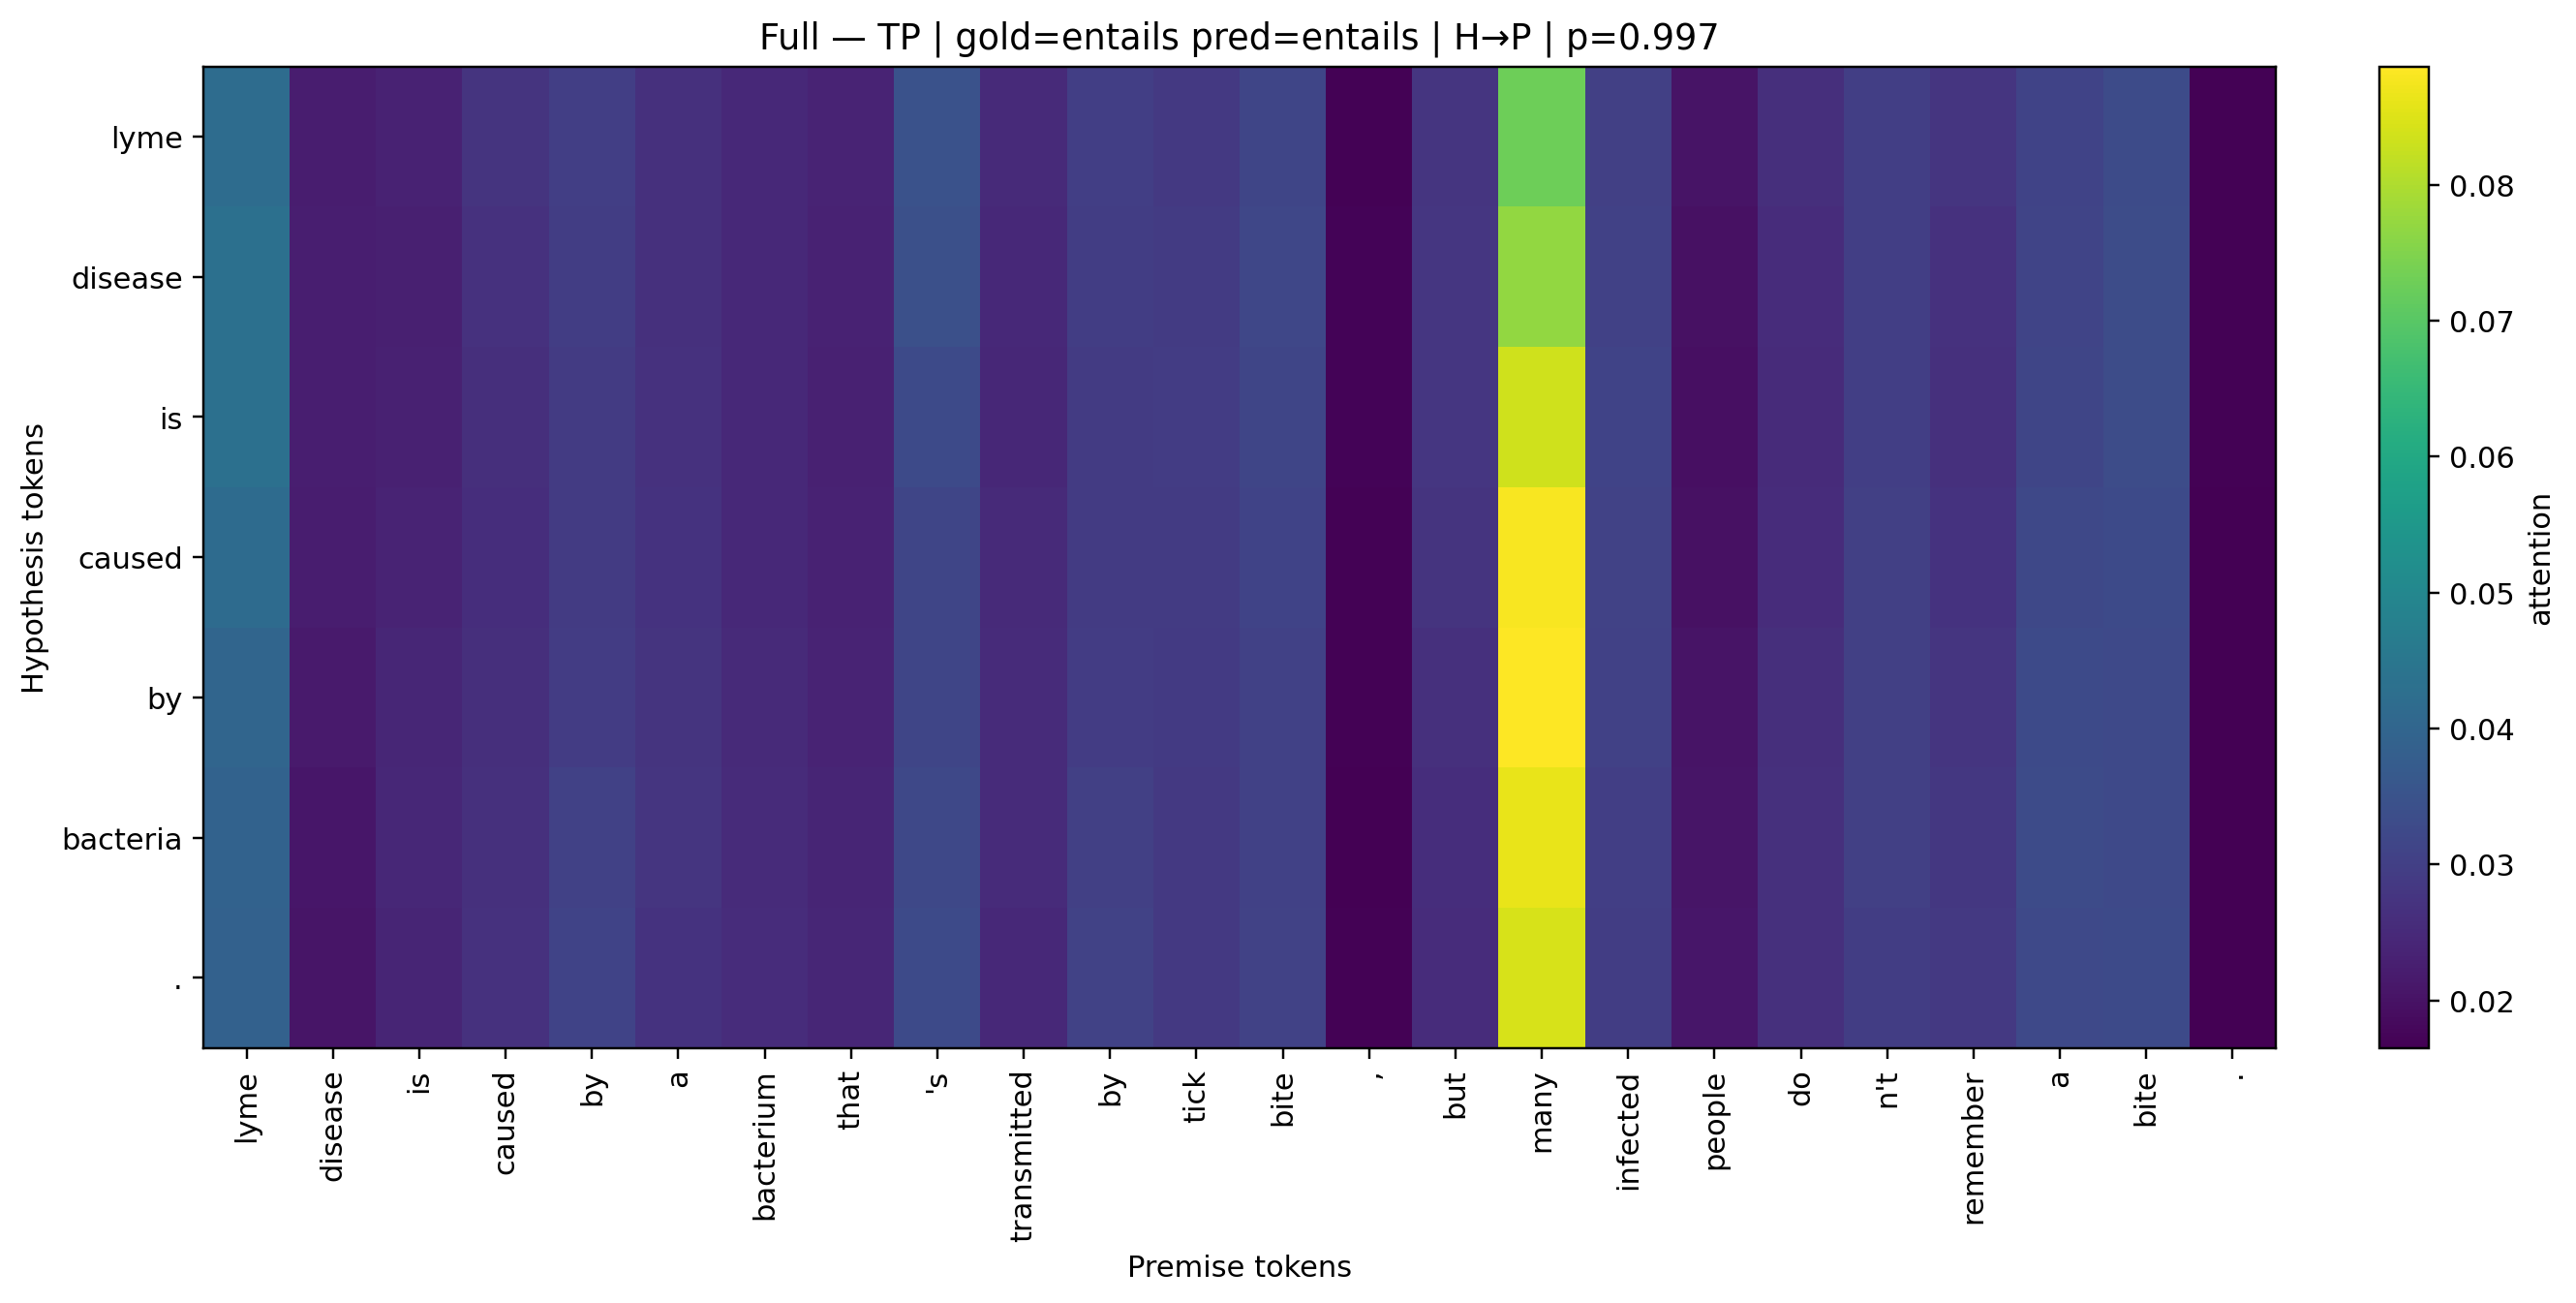
\includegraphics[width=\linewidth]{full_TP_y-entails_pred-entails_p-0.997_H2P.png}
    \caption{Full — TP}
    \label{fig:full-tp}
  \end{subfigure}\hfill
  \begin{subfigure}{0.49\linewidth}
    \centering
    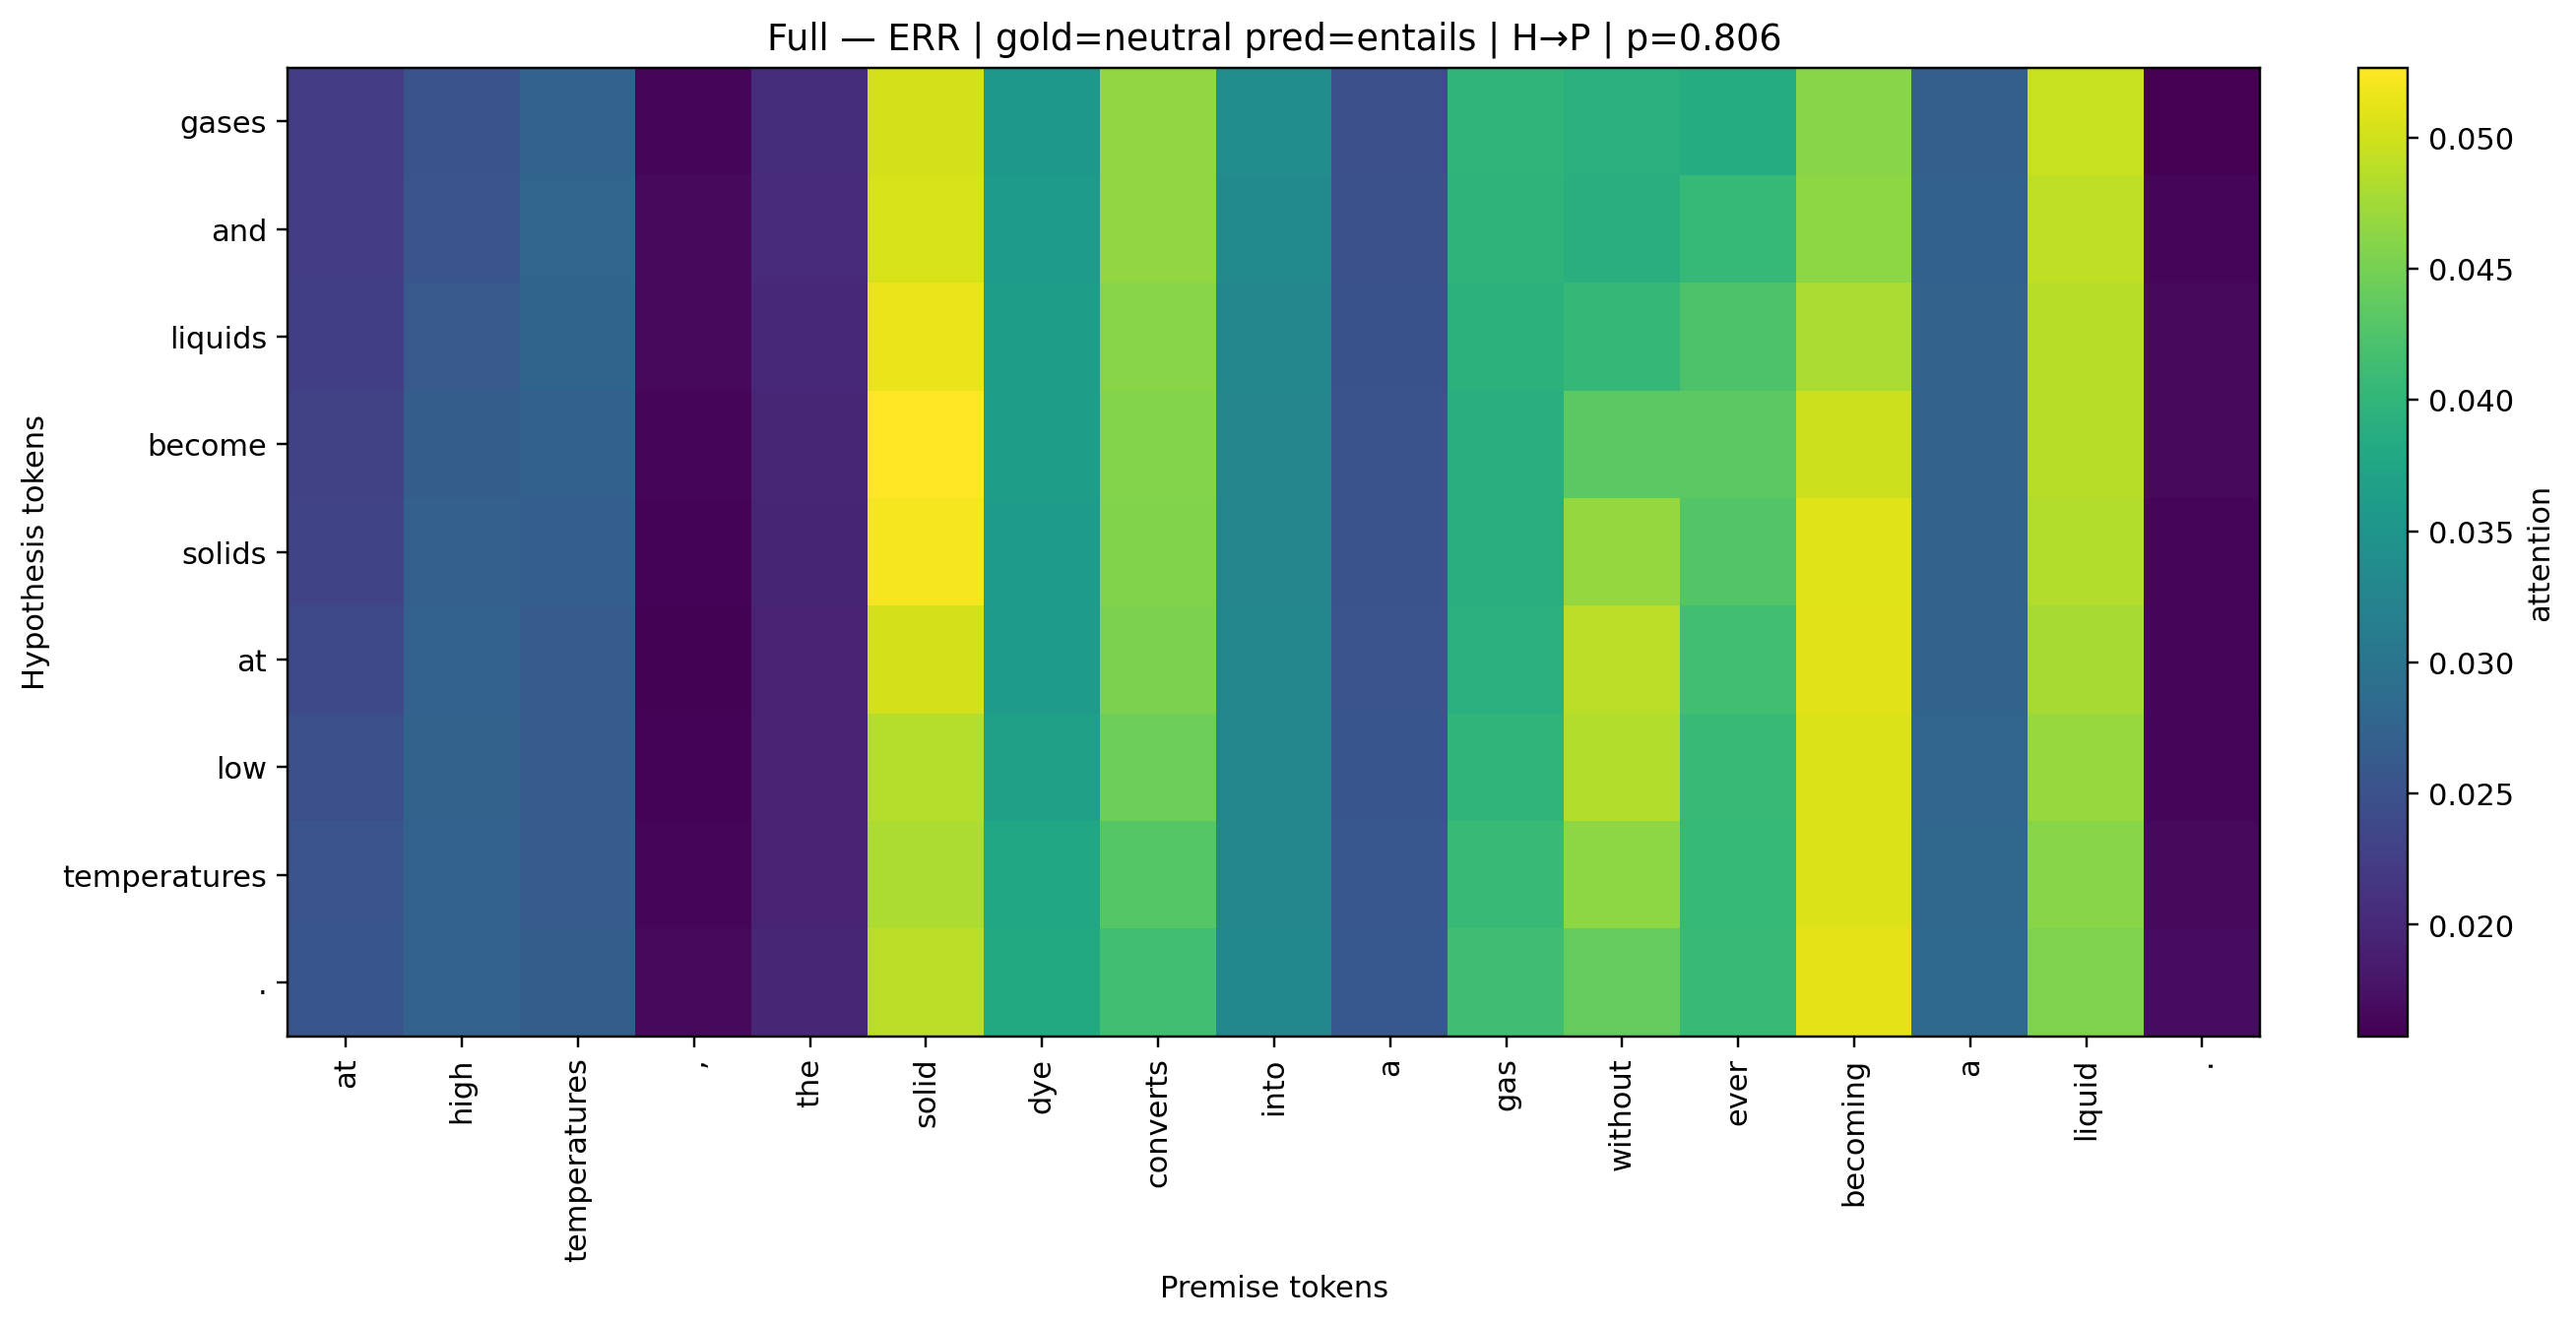
\includegraphics[width=\linewidth]{full_ERR_y-neutral_pred-entails_p-0.806_H2P.png}
    \caption{Full — FP}
    \label{fig:full-fp}
  \end{subfigure}
  \caption{\textit{Full} model: TP vs.~FP.}
  \label{fig:full-pair}
\end{figure}
\FloatBarrier
\FloatBarrier
% ---------- C→P only: TP vs FP ----------
\begin{figure}[!htbp]
  \centering
  \begin{subfigure}{0.49\linewidth}
    \centering
    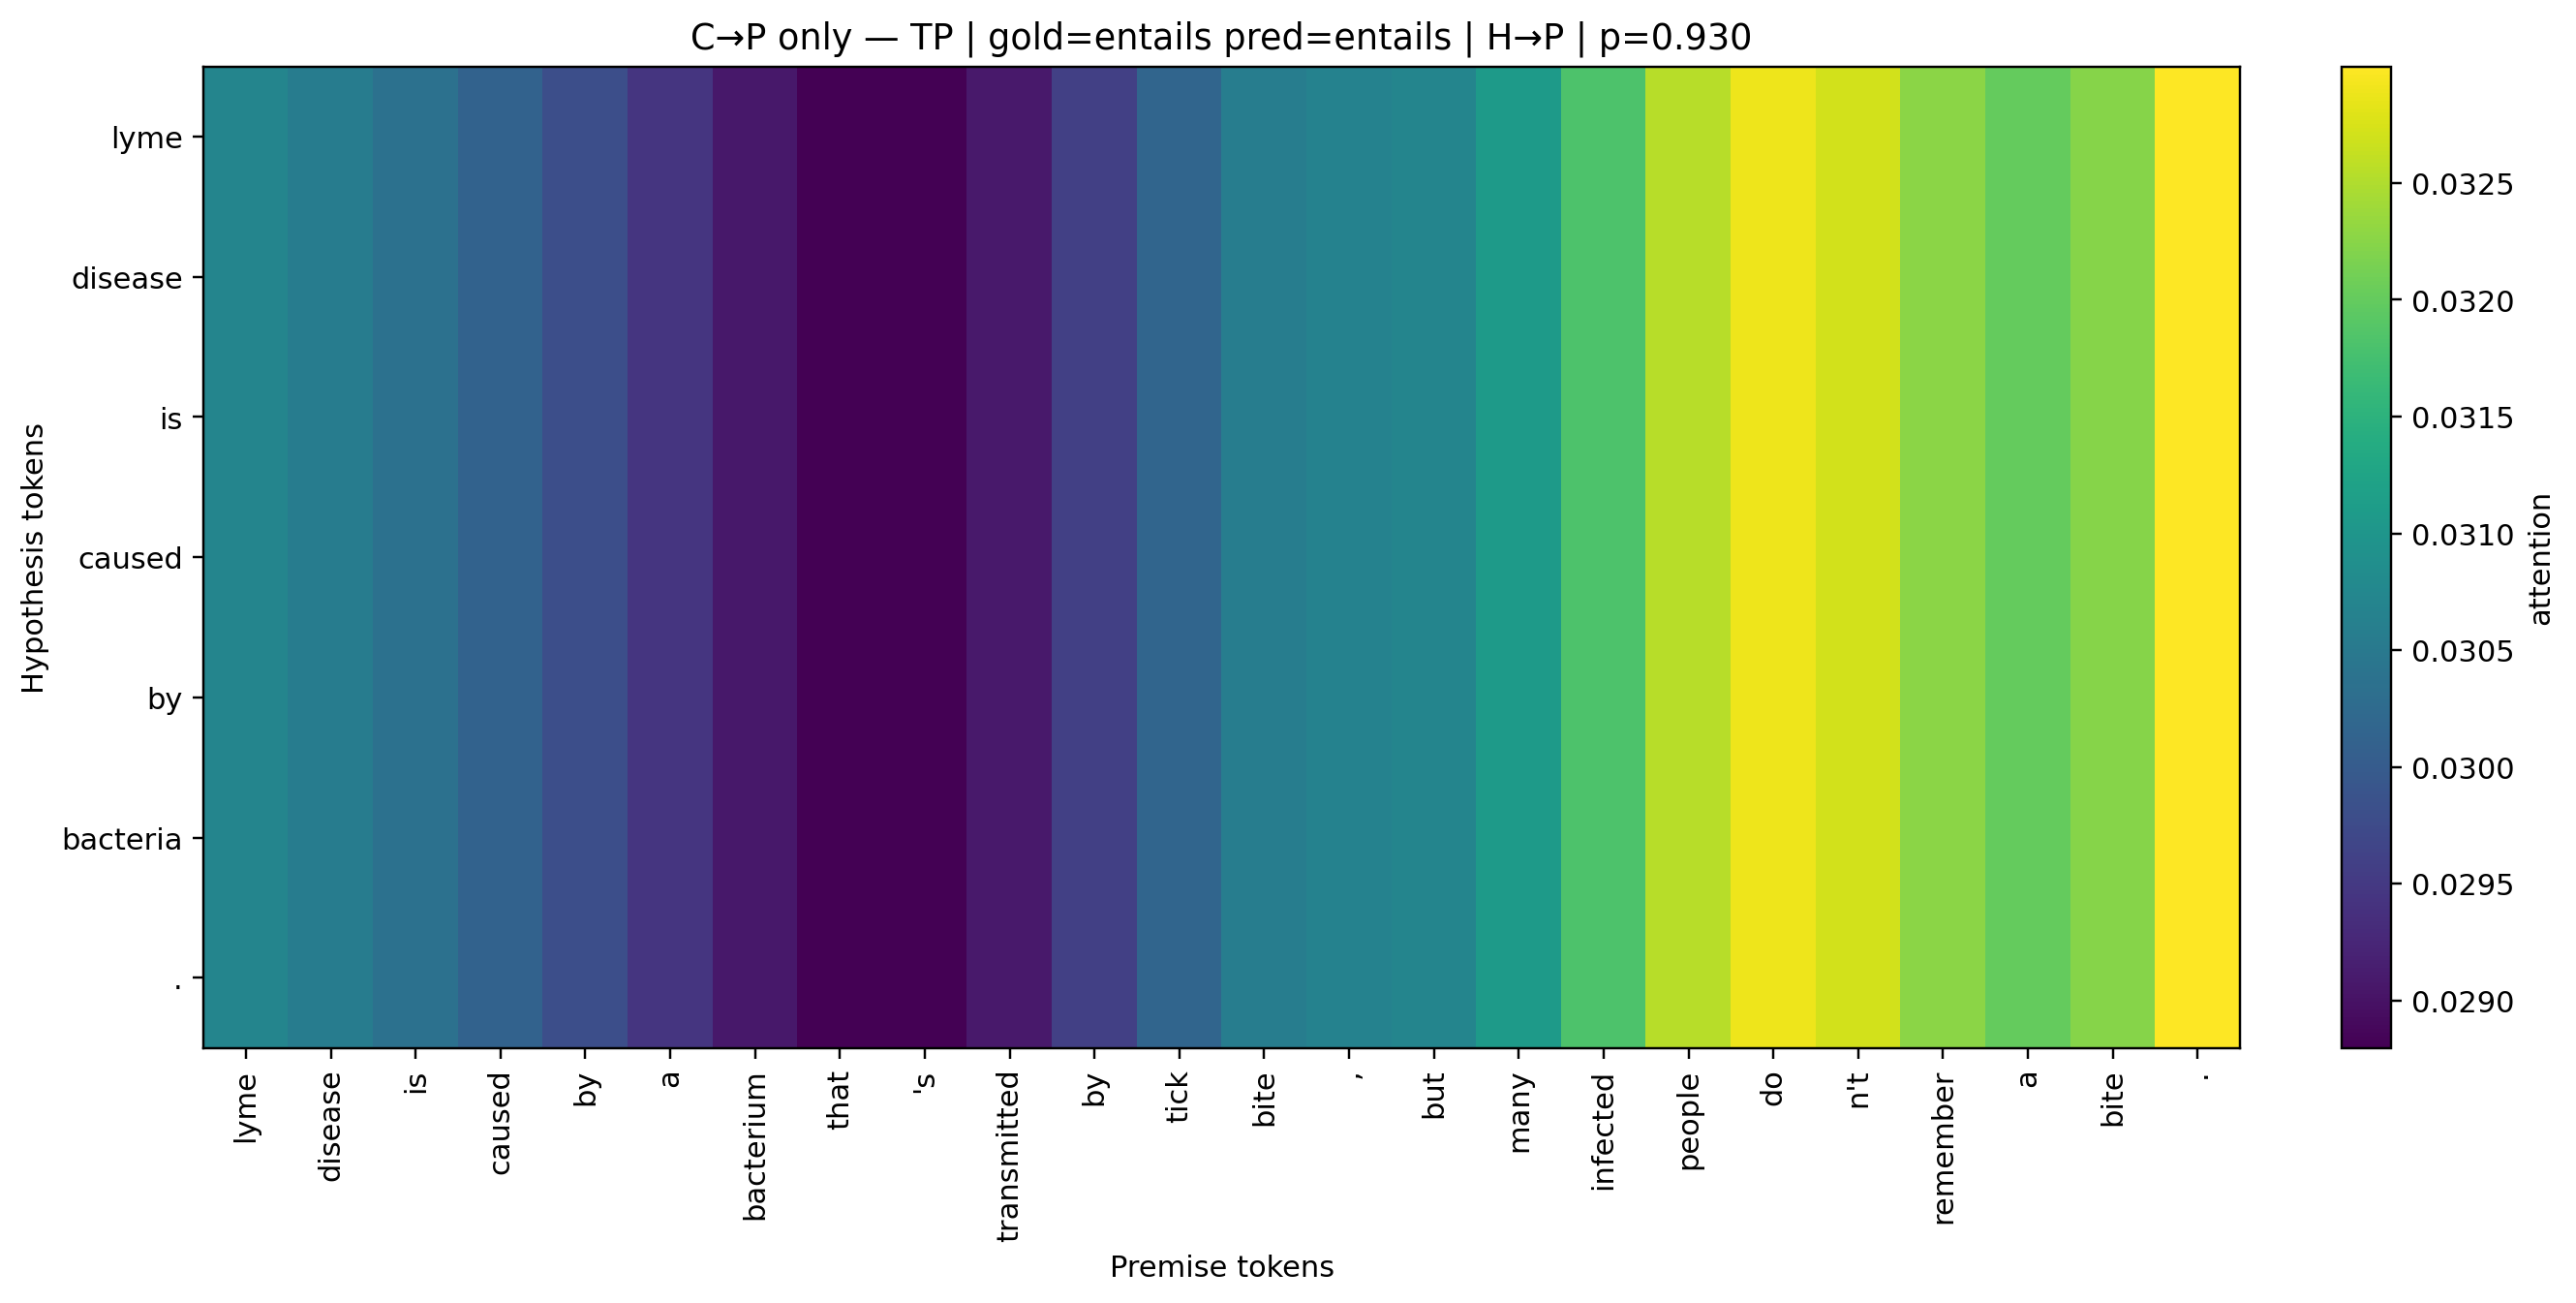
\includegraphics[width=\linewidth]{c2p_only_TP_y-entails_pred-entails_p-0.930_H2P.png}
    \caption{C$\to$P only — TP}
    \label{fig:c2p-tp}
  \end{subfigure}\hfill
  \begin{subfigure}{0.49\linewidth}
    \centering
    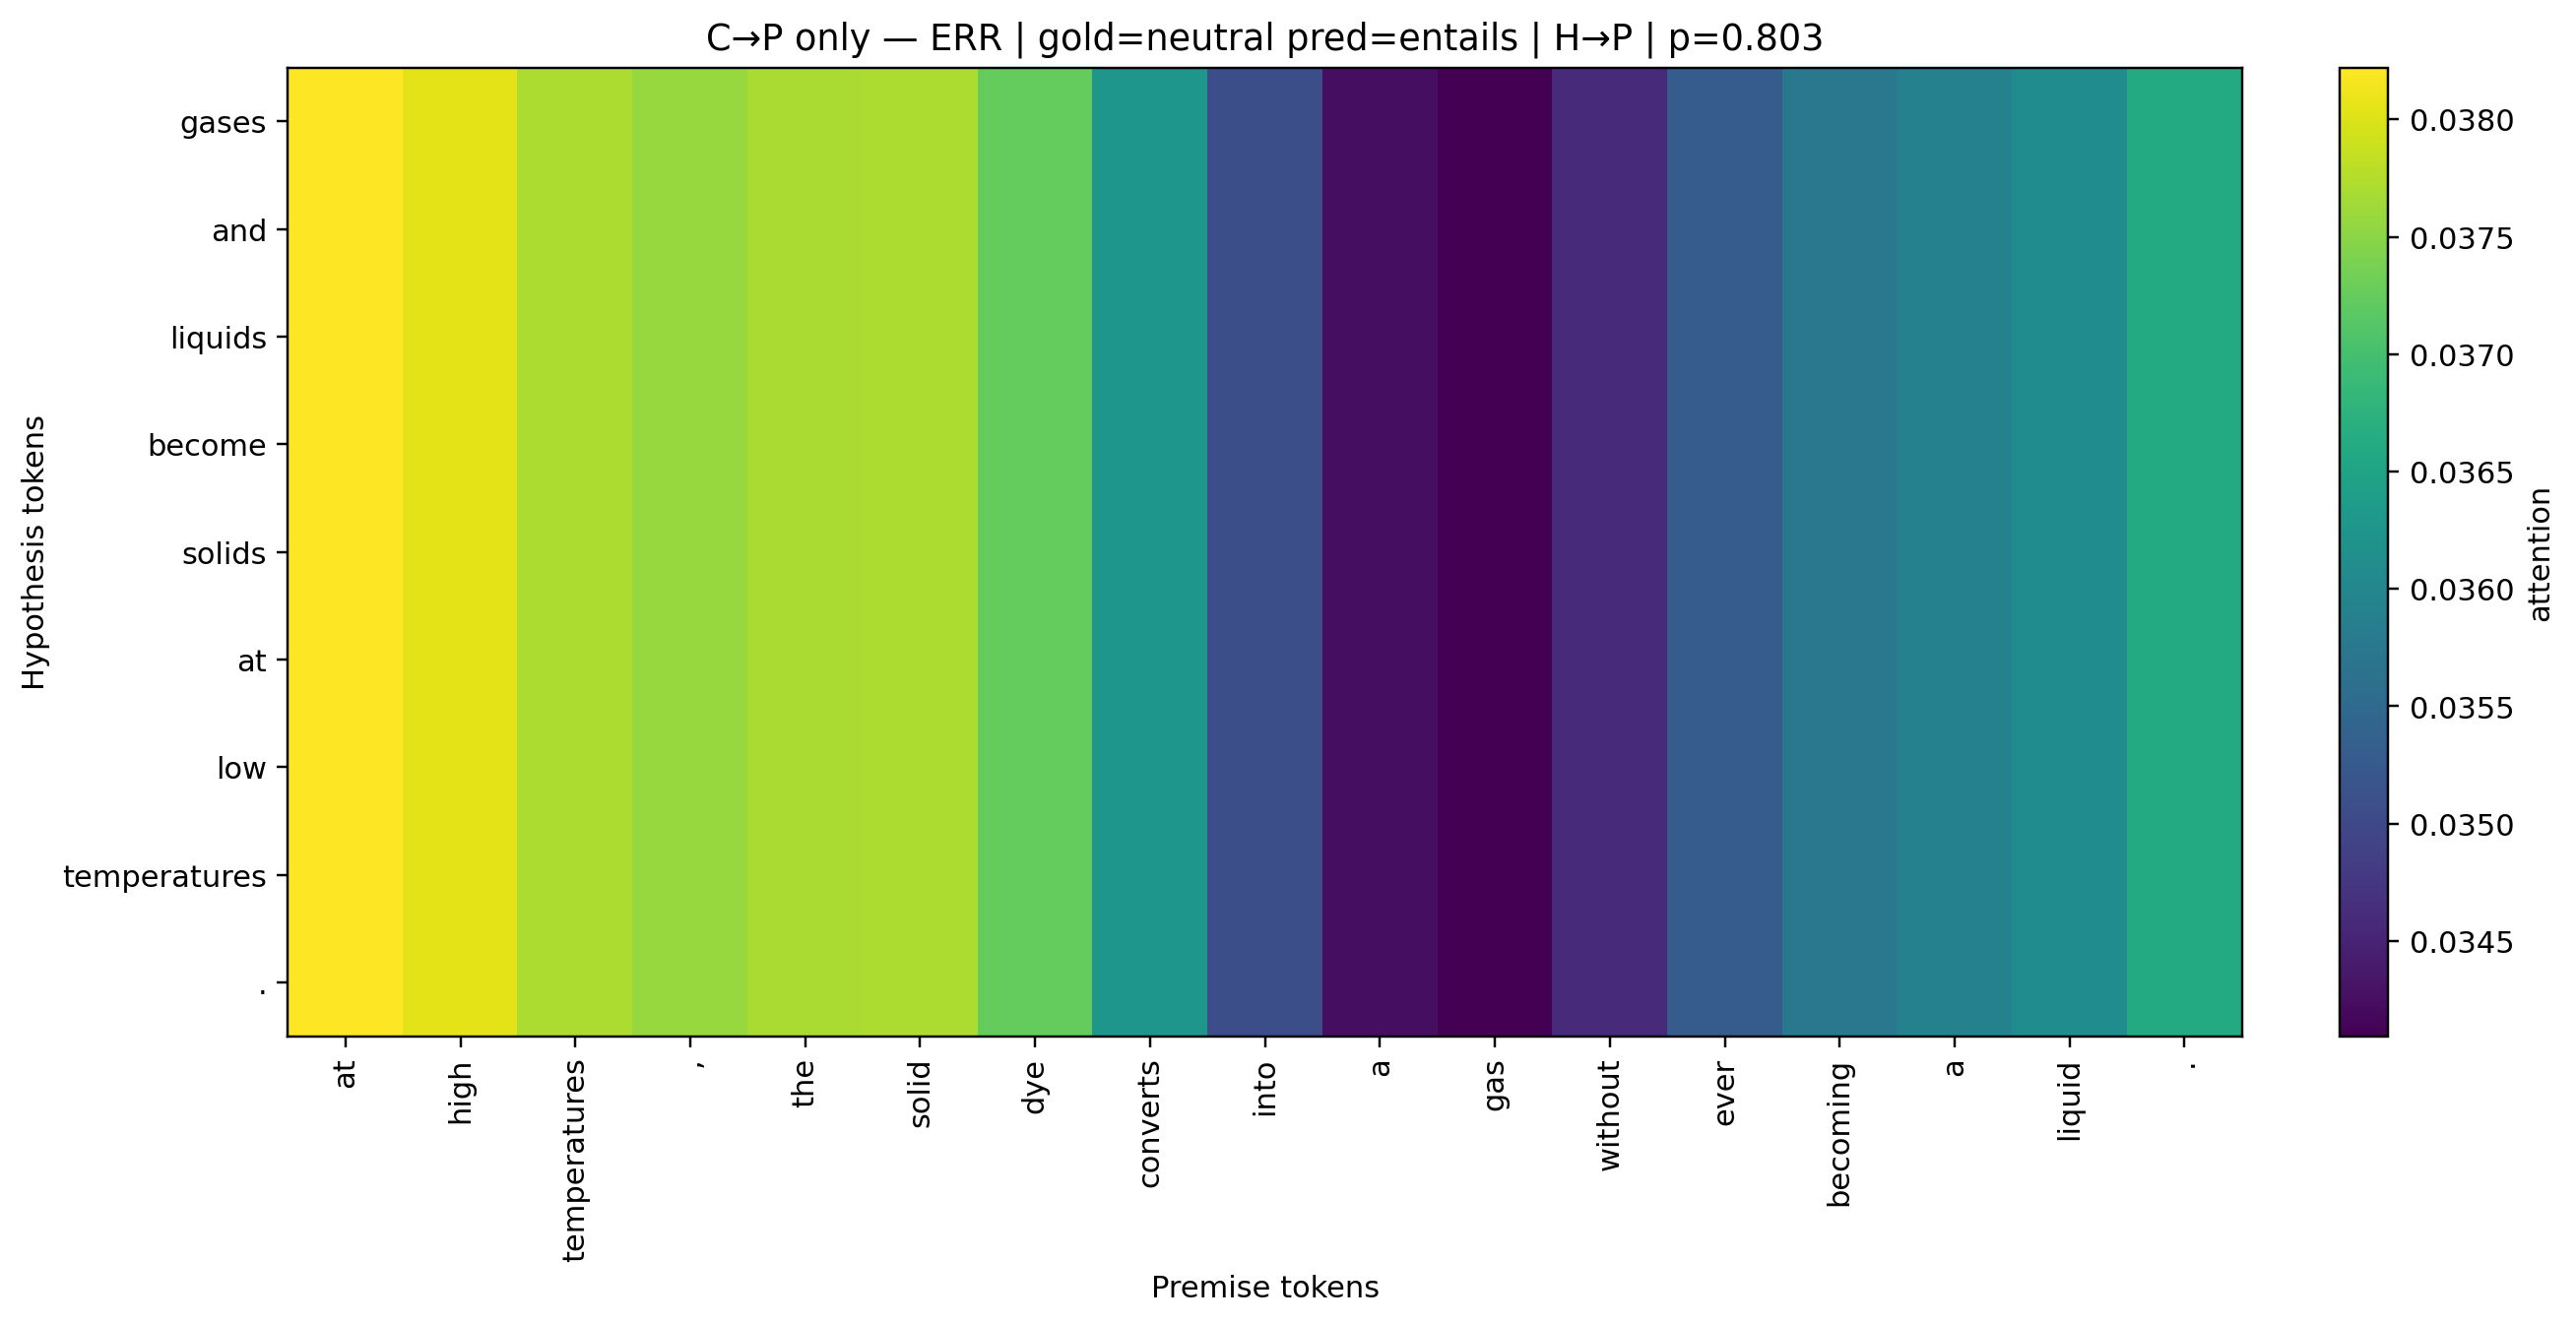
\includegraphics[width=\linewidth]{c2p_only_ERR_y-neutral_pred-entails_p-0.803_H2P.png}
    \caption{C$\to$P only — FP}
    \label{fig:c2p-fp}
  \end{subfigure}
  \caption{C$\to$P only model: TP vs.~FP.}
  \label{fig:c2p-pair}
\end{figure}
\FloatBarrier

\end{document}

